\thispagestyle{empty}
\chapter{Discussion générale}
{\hypersetup{linkcolor=GREYDARK}\minitoc}
\label{chap:discuss-general}


\section{Résumé des principaux résultats}

Au cours de mes travaux de thèses, nous avons vu que tout le long de l'histoire évolutive des espèces, l'intégration accidentelle d'éléments viraux dans le génome eucaryote peut se produire \citep{katzourakis_endogenous_2010}. Ces éléments peuvent parfois conférer aux génomes receveurs des avantages évolutifs majeurs : on parle alors de domestication virale. Par exemple, chez certaines guêpes endoparasitoïdes (dont les stades immatures se développent à l'intérieur de leurs hôtes), la propriété fusogènique des virus a été domestiquée à plusieurs reprises suite à des intégrations virales ancestrales de virus dsDNA. Ces gènes viraux endogénisés sont utilisés par les guêpes femelles comme un outil pour injecter des facteurs de virulence, essentiels au succès du développement de leur progéniture \citep{drezen_endogenous_2017}. Comme tous les cas connus de domestication virale impliquent des guêpes endoparasitoïdes \citep{bezier_polydnaviruses_2009,volkoff_analysis_2010,pichon_recurrent_2015,burke_common_2019,di_giovanni_behavior-manipulating_2020}, nous avons au début de ma thèse émis l'hypothèse que ce mode de vie (favorisant une interaction étroite entre les individus) pouvait favoriser l'endogénisation et la domestication de virus. Ainsi, en analysant la composition génomique de 124 génomes d'Hyménoptères répartis dans la diversité des Hyménoptères et incluant des espèces libres, ecto et endoparasitoïdes, nous avons testé cette hypothèse dans le \hyperref[sec:chap1]{chapitre 1}. Notre analyse a d'abord révélé que les virus à ADN double brin étaient plus souvent endogénisés et domestiqués que prévu d'après leur abondance relative estimée dans les communautés virales infectant les insectes par rapport aux autres structures génomiques virales (ssDNA, dsRNA, ssRNA). Deuxièmement, notre analyse a révélé que l'endogénisation et la domestication des virus à ADN double brins étaient plus fréquentes dans les espèces ayant un mode de vie endoparasitoïde par rapport aux espèces ayant un mode de vie ectoparasitoïde ou libre. Ces résultats suggèrent donc que l'endoparasitoïsme a promu la domestication des virus à ADN double brins ou inversement que la domestication de ces virus a favorisé l'évolution de l'endoparasitoïsme.\\
 
Deuxièmement, dans un projet collaboratif avec l'équipe de l'IRBI de Tours, j'ai pu exploiter les données dites "exogènes" de mon premier projet pour décrire cette fois-ci plutôt de nouveaux virus infectieux présents dans des assemblages de génomes de guêpes parasitoïdes. Nous avons en particulier recherché la présence de virus à allure filamenteuse apparentés au virus retrouvé chez l'espèce parasitoïde \textit{Leptopilina boulardi}. Ce virus connu pour manipuler le comportement du parasitoïde est actuellement le seul représentant d’une probable nouvelle famille de virus à ADN. C'est ainsi qu'au cours de ce projet, nous avons pu caractériser cette nouvelle famille virale en analysant le contenu en gènes et l’histoire évolutive de 7 nouveaux génomes de virus appartenant à cette famille. Ce travail constitue ainsi la base préliminaire pour leur classification dans l'ICTV comme une nouvelle famille que nous proposons de nommer Filamentoviridae en raison de leur structure filamenteuse singulière, créant ainsi une cinquième famille de la classe \textit{Naldaviricetes} des virus à ADN double brins. Ces résultats tendent également à montrer que ces virus sont préférentiellement associés à des espèces de guêpes endoparasitoïdes dont le style de vie particulier a très probablement permis à ces virus de se transmettre efficacement entre générations.\\
 
Enfin, la dernière partie de mon doctorat consistait à étudier les EVEs dans un clade de guêpes endoparasitoïdes initialement identifié dans notre laboratoire (Di Giovanni et al., 2020). Ce clade correspond aux espèces du genre \textit{Leptopilina}, chez qui 13 gènes provenant de la famille des Filamentoviridae ont été domestiqués et participent à la production de particules virales qui protègent les œufs des guêpes du système immunitaire de leur hôte. Mes résultats indiquent qu'un événement d'endogénisation et de domestication virale s'est produit il y a environ 75 millions d'années chez l'ancêtre commun de la majorité des espèces de guêpes appartenant à la tribu des Eucoilini (contenant les \textit{Leptopilina}). L'endogénisation de ces gènes correspond à la période de diversification des hôtes de ces guêpes parasitoïdes, ce qui suggère que la domestication des gènes viraux ait pu aider les guêpes à s'adapter à leurs hôtes à cette époque. Par ailleurs, nous mettons également en évidence un nouvel évènement indépendant ayant probablement donné lieu au remplacement d'un gène provenant du premier évènement chez l'espèce \textit{Rhoptromeris}. Enfin, la caractérisation temporelle du premier événement d'endogénisation ancestral au sein des Eucoilini nous a permis de calibrer la phylogénie des Filamentoviridae. Cette calibration nous permet d'estimer que la diversification des Filamentoviridae a eu lieu, il y a environ 297 millions d'années, ce qui correspond à peu près au moment de l'apparition des Hyménoptères. Par la suite, au cours de l'évolution, ces virus se seraient ensuite préférentiellement associés aux lignées d'Hyménoptères ayant un mode de vie endoparasitoïde.\\ 

%coïnciderait à nouveaux avec l'hypothèse initiale que ces virus sont intrinsèquement liés à ce mode de vie.  \\

%Ces trois chapitres abordent plusieurs questions sur plusieurs échelles évolutives. Au-delà de la discussion de chacun de ces travaux, nous pouvons donc tenter de discuter plus largement des implications de ces résultats et ce qu'ils peuvent nous apprendre de la biologie et l'évolution des espèces endoparasitoïdes et des virus avec lesquels elles interagissent depuis des millions d'années. \\


\section{Pourquoi les phénomènes de domestication sont-ils plus fréquents chez les espèces endoparasitoïdes et impliquent préférentiellement les virus dsDNA?}

Dans le \hyperref[sec:chap1]{chapitre 1}, nous mettons en évidence que le mode de vie endoparasitoïde favorise davantage les événements d'endogénisation et de domestication des virus dsDNA que les modes de vie ectoparasitoïde ou libre. Plusieurs questions se posent à la suite de ces observations. Pourquoi ce phénomène est-il limité aux virus dsDNA ? Pourquoi le mode de vie endoparasitoïde est-il préférentiellement associé à de tels événements, et quels effets, le cas échéant, ces évènements de domestication ont-ils sur la biologie de ces espèces ?\\

\textbf{H1 - Un plus grand input en virus chez les endoparasitoïdes?}

Comme première hypothèse pour comprendre ces observations, nous pourrions imaginer que l'écologie particulière des espèces endoparasitoïdes  en interaction étroite avec leur hôte soit associée à un plus grand nombre d'opportunités d'intégrations virales accidentelles. En effet, des endoparasitoïdes peuvent être plus intensivement exposés aux virus comparé à d'autres Hyménoptères au style de vie ectoparasitoïde ou bien libre.

De multiples éléments viennent étayer cette hypothèse. Les larves endoparasitoïdes se développent par définition à l'intérieur du corps de leur hôte, et une interaction aussi étroite implique que tout individu endoparasitoïde interagira également avec les virus de son hôte. En appui à cette idée, il est intéressant de noter que la plupart des cas de domestication de virus par les  guêpes endoparasitoïdes impliquent les nudivirus. Les virus de cette famille infectent en effet les Lépidoptères qui sont les hôtes des parasitoïdes en question \citep{burke_rapid_2018,pichon_recurrent_2015,bezier_polydnaviruses_2009-1}. Un autre facteur important est la présence de virus dans les venins que les endoparasitoïdes injectent dans les hôtes au côté de leurs œufs. La présence de ces virus dans ces compartiments pourrait favoriser la propagation ultérieure des virus dans les populations de guêpes. Par exemple, en colonisant les tissus producteurs de venin (glande venimeuse ou calice, selon la biologie de l'espèce), les virus peuvent assurer une transmission pseudo-verticale efficace et ainsi se maintenir efficacement dans les populations de guêpes. De nombreux virus endoparasitoïdes bénéficient d'une telle transmission pseudo-verticale \citep{varaldi_artifical_2006,renault_cypovirus_2003,coffman_viral_2022}, dont certains ont été domestiqués par les endoparasitoïdes (ou tout du moins leurs ancêtres) (Di Giovanni et al., 2020). La présence de virus dans les venins peut également faciliter la transmission horizontale au sein des espèces en cas de superparasitisme, par exemple chez le virus filamenteux de \textit{Leptopilina boulardi} infectant des drosophiles \citep{varaldi_infectious_2003} ou bien l'entomopoxvirus chez \textit{Diachasmimorpha longicaudata} infectant des larves de mouches des fruits téphritides \citep{coffman_viral_2022}, ou bien encore un ascovirus mutualiste (DpAV4) chez plusieurs espèces du genre \textit{Diadromus} \citep{stasiak_characteristics_2005}. On peut donc s'attendre à une prévalence de virus plus élevée  chez les endoparasitoïdes par rapport aux autres Hyménoptères, ce qui peut expliquer en partie le fait que les espèces endoparasitoïdes intègrent puis domestiquent plus fréquemment des éléments viraux. 

Cependant, si cette explication était la bonne, nous devrions observer davantage d'intégration et de domestication chez les espèces endoparasitoïdes pour tous les virus recherchés. Au contraire, nos résultats ne révèlent ce schéma que pour les virus à ADN double brin. Nous pensons donc qu'un processus plus complexe est à l'œuvre, incluant l'interaction de deux facteurs (le mode de vie et le type de virus). \\

\textbf{H2 - les endoparasitoïdes "retiennent" les EVEs plus fréquemment, car ils leur confèrent un avantage}

Par conséquent, une deuxième hypothèse peut aider à expliquer ces données. Cette hypothèse propose que les endoparasitoïdes sélectionnent plus fréquemment les gènes viraux endogénisés provenant de virus dsDNA, car ces gènes apportent un avantage évolutif à ces guêpes spécifiquement.\\

À ce propos, dans le \hyperref[sec:chap1]{chapitre 1}, nous avons effectivement observé que les guêpes endoparasitoïdes présentaient plus fréquemment des évènements de domestication de virus dsDNA comparé aux espèces libres ou ectoparasitoïdes. Il est clair que cela peut s'expliquer en partie par un taux d'endogénisation plus élevé (H1), ce qui expliquerait également un taux de domestication plus élevé. Après avoir corrigé cet effet en corrélant le nombre d'événements de domestication avec le nombre d'événements d'endogénisation, une tendance vers un taux de domestication plus élevé demeure (\figurename{\ref{figure:dsDNA_violin_plots_corrected_rates}}). Plus précisément, la probabilité de domestication après endogénisation était plus grande pour les endoparasitoïdes que pour les ectoparasitoïdes, mais pas significativement plus grande que pour les espèces libres. Ce manque de signification statistique pourrait être biologiquement explicable si l'on suppose qu'un événement de domestication empêche l'apparition d'événements de domestication ultérieurs sans influencer le taux d'endogénisation non adaptatif. Cela aurait pour effet de " diluer " le signal le long des branches liées à la domestication. Si cet impact est en jeu, alors notre capacité à remarquer les différences de taux de domestication entre les modes de vie est fortement affaiblie.  En effet, pour les six cas de domestications décrits dans la littérature, à chaque fois, un unique virus "donneur" a été domestiqué. Ceci suggère que des domestications supplémentaires ne soient pas avantageuses après qu'une lignée de guêpes a recruté une machinerie virale. Le seul exemple de remplacement d'une machinerie virale entière serait chez \textit{V. canescens}, où un ichnovirus (polydnavirus) aurait été remplacé par un nudivirus (VLPs) \citep{pichon_recurrent_2015}. Cependant, l'analyse faite dans le \hyperref[sec:chap1]{chapitre 1} (qui incluait \textit{V. canescens}), n'a pas permis de confirmer ce remplacement.\\

Nous pouvons maintenant discuter des avantages de sélection que pourraient fournir les EVEs chez les endoparasitoïdes comparé aux autres hyménoptères.\\ 

En termes d'interactions, alors que les guêpes ectoparasitoïdes utilisent leur venin pour conserver la nourriture pour leurs progénitures, les guêpes endoparasitoïdes utilisent leur venin pour transformer les organismes en pouponnières où leur progéniture pourra vivre et se nourrir à l'éclosion \citep{moreau_chapter_2009,schendel_diversity_2019}. De plus, plusieurs études montrent que les espèces ectoparasitoïdes interagissent moins avec le système immunitaire de leurs hôtes comparé à des espèces au style de vie endoparasitoïde \citep{li_parasitism_2018}. Par exemple, le venin de l'ectoparasitoïde \textit{Scleroderma guani} inhibe moins efficacement l'encapsulation que les venins d'autres endoparasitoïdes \citep{cai_parasitism_2004, richards_venom_2000}. Ou bien, il a également été mis en évidence que l'ectoparasitoïde \textit{Nasonia} pouvait développer sa progéniture sans le venin que la femelle injecte normalement, bien qu'il puisse être tout de même bénéfique pour les progénitures \citep{martinson_venom_2018}. Au contraire, les venins injectés par plusieurs espèces d'endoparasitoïdes sont absolument nécessaires pour contourner la réponse immunitaire de l'hôte \citep{guillot_rocalyx_1972,li_parasitism_2018, lee_chapter_2009, small_introduction_2012}. Cela pourrait être dû au fait que les œufs de guêpes ectoparasitoïdes ne se développent pas à l'intérieur de la cavité de l'hôte, ce qui signifie que les protéines actives du venin impliquées dans la prévention de l'encapsulation des hémocytes ne sont pas strictement nécessaires à la survie de ces parasitoïdes \citep{li_parasitism_2018}. Les espèces endoparasitoïdes sont quant à elles plus exposées au système immunitaire de l'hôte puisqu'elles se retrouvent lors de la ponte à l'intérieur du corps de son hôte et notamment dans l'hémocoele là où transite toutes les cellules immunitaires. Il est donc plausible que les organismes endoparasitoïdes soient effectivement soumis à des pressions de sélection bien plus élevées de la part du système immunitaire de leurs hôtes que les espèces ectoparasitoïdes \citep{li_parasitism_2018}.\\

Aussi, toute stratégie permettant aux guêpes endoparasitoïdes de lutter efficacement contre le système immunitaire de l'hôte devrait être fortement sélectionnée au cours de l'évolution. Parmi les stratégies connues, il existe, comme nous l'avons vue, plusieurs qui font intervenir des virus endogénisés. En effet, des virus, exclusivement dsDNA, ont été endogénéisés et domestiqués à plusieurs reprises par des endoparasitoïdes \citep{bezier_polydnaviruses_2009,volkoff_analysis_2010,pichon_recurrent_2015,burke_common_2019,di_giovanni_behavior-manipulating_2020}. Dans ce cas, les parasitoïdes ont coopté la propriété fusogénique de ces virus pour adresser des structures à allures virales (VLS) sous forme de protéines (VLP) ou d'ADN (polydnavirus) aux cellules immunitaires de leurs hôtes, inhibant ainsi la réponse immunitaire cellulaire. Aussi, nous pourrions faire l'hypothèse que chez ces espèces endoparasitoïdes, ce type d'évènements devraient être plus fréquemment sélectionné comparé aux autres styles de vie. Et ceci, car la production de VLS devrait participer grandement au succès parasitaire chez ces guêpes en adressant des facteurs de virulence qui vont désactiver les cellules immunitaires des hôtes. Ces observations pourraient donc êtres liés par ce phénomène qui implique que le style de vie endoparasitoïde aurait plus fréquemment domestiqués des virus dsDNA car ceux-ci permettraient, via la production de VLS, de faire face aux pressions sélectives liées au système immunitaire de leurs hôtes. 

Seulement, lors du \hyperref[sec:chap1]{chapitre 1}, nous n'avons identifié qu'un seul cas de domestication ressemblant à ceux déjà décrits (impliquant la domestication de toute une batterie de gènes viraux) chez \textit{Platygaster orseoliae}. Nous pourrions donc nous demander si toute une batterie de gène est strictement nécessaire à la production effective de ces VLS. En effet, dans notre analyse du \hyperref[sec:chap1]{chapitre 1}, le driver principal de "l'effet endoparasitoïde" de ces phénomènes de domestications concerne essentiellement des évènements comportant un ou deux gènes. \\

À cela, nous pourrions donc supposer que des fonctions supplémentaires totalement distinctes nécessitant un petit nombre de gènes soient également adaptatifs pour ces guêpes particulièrement. Par exemple, chez les pucerons du pois, la domestication de deux gènes de densovirus seulement est impliquée dans la plasticité du phénotype ailé \citep{parker_laterally_2019}. Ou bien chez les mammifères placentaires et des lézards vivipares, un seul gène \textit{env} rétroviral est impliqué dans la formation du syncitium \citep{lavialle_paleovirology_2013,cornelis_endogenous_2017}.\\

\textbf{Mais pourquoi spécifiquement les virus dsDNA?}

Dans un premier temps, nous pourrions imaginer que les virus à ADN double brins seraient plus à même à rentrer dans les génomes que les hôtes compte tenu du fait qu'ils présentent des génomes de même structure que ceux des guêpes et que la plupart se répliquent dans le noyau de leurs hôtes. En effet, la réplication nucléaire est une caractéristique partagée par presque toutes les familles de virus dsDNA trouvées dans notre analyse, à l'exception des \textit{Poxviridae}, qui se répliquent dans le cytoplasme. De plus, puisque ces cas de domestication indépendants sont exclusifs aux virus dsDNA, il est possible que ces virus aient un meilleur potentiel de transmission de facteurs de virulence par rapport aux autres virus. Dans quelques cas connus, il semble qu'une façon de délivrer efficacement des facteurs de virulence à la cellule hôte consiste à adresser des cercles d'ADN (dans les polydnavirus que l'on trouve chez certains Braconidae et Campopleginae) qui s'intègrent finalement dans les cellules immunitaires de l'hôte et s'expriment \citep{chevignon_functional_2014, chevignon_cotesia_2018}. L'ADN qui est emballé dans les particules matures provient de l'hôte et code généralement pour des protéines de virulence provenant de la guêpe \citep{espagne_genome_2004,burke_widespread_2014}. Cela signifie qu'au moins dans ces cas, le système viral devrait être capable d'emballer des cercles d'ADN de 180 à plus de 600kb \citep{burke_polydnaviruses_2012}, ce qui est très probablement une caractéristique que possèdent les EVEs dérivés de virus à ADN. Cependant, d'autres systèmes décrits ne reposent pas sur l'emballage de l'ADN, mais plutôt sur l'emballage des protéines de virulence (dans les systèmes dits VLPs). La raison pour laquelle les EVEs dérivées de virus à ADN seraient plus aptes à le faire n'est pas claire. Cependant, une caractéristique majeure qui distingue les virus dsDNA des autres virus est clairement la taille de leur génome et, corrélativement, la taille de leur capside et de leur enveloppe, qui est beaucoup plus grande \citep{chaudhari_scaling_2021}. Cela pourrait prédisposer les virus dsDNA à être domestiqués, puisque d'abondantes quantités de venins ou bien de cercles d'ADN doivent être transmises afin de supprimer efficacement la réponse immunitaire de l'hôte \citep{beckage_parasitoid_2008}. \\


Enfin, d'autres fonctions pourraient également êtres en œuvre parmi ces EVEs comme celle de conférer une immunité antivirale contre des virus apparentés "libres" via la voie des ARNi \citep{suzuki_non-retroviral_2020,whitfield_diversity_2017}. Cependant, bien que cette hypothèse soit plausible, elle ne peut expliquer les données que si les virus dsDNA bénéficient mieux de cet effet par rapport aux autres structures génomiques. Au contraire, à notre connaissance, l'immunité antivirale conférée par les EVEs n'a été démontrée que contre des virus à ARN, mais pas contre des virus à ADN \citep{ter_horst_endogenous_2019}. De plus, les identités de séquences avec des séquences virales connues, qui sont nécessaires pour que ce mécanisme fonctionne, sont faibles dans l'ensemble de nos données. Des travaux antérieurs ont d'ailleurs révélé que les piRNA dérivés des EVEs étudiés chez 48 espèces d'arthropodes étaient aussi probablement trop divergents pour induire une réponse antivirale efficace \citep{ter_horst_endogenous_2019}. Il est donc peu probable que ces EVEs puissent générer des ARNs interagissant avec le PIWI et jouer un rôle fonctionnel dans l'immunité antivirale. Pour faire la lumière sur cette question, des recherches supplémentaires utilisant le séquençage de petits ARN chez les espèces d'hyménoptères seraient nécessaires. \\

D'autres fonctions pourraient aussi concerner des gènes viraux avec des fonctions encore inconnues, mais facilitant aussi le succès parasitaire par d'autres moyens, comme par exemple les gènes de virus dsDNA (PKF) qui sont au contraire utilisés par les hôtes Lépidoptères pour éliminer les parasitoïdes \citep{gasmi_horizontally_2021}. Quoi qu'il en soit, il est évident que cette dernière idée mérite des investigations supplémentaires, notamment sur la fonction spécifique des EVEs et leur contribution potentielle au succès reproductif des guêpes.\\

\section{L'endoparasitoïdisme comme moteur de la domestication, ou bien la domestication comme moteur de l'endoparasitoïdisme?}

Nous l'avons vu en introduction, la transition vers le mode de vie parasitoïde ne se serait produite qu'une seule fois, il y a environ 247 millions d'années, suivie de quelques réversions importantes \citep{peters_evolutionary_2017}. Ce mode de vie aurait ensuite évolué au cours du temps, donnant notamment naissance aux ectoparasitoïdes et aux endoparasitoïdes (avec probablement de multiples transitions entre ces deux états). Nous pourrions alors nous demander, au vu de nos résultats, si le style de vie endoparasitoïdes serait apparu grâce à la domestication virale (hypothèse 1), ou bien si, au contraire, ce style de vie déjà bien établi aurait plutôt facilité les évènements de domestication de virus (hypothèse 2). 

\begin{figure}[H]
\captionsetup{font=footnotesize}
 \centering
  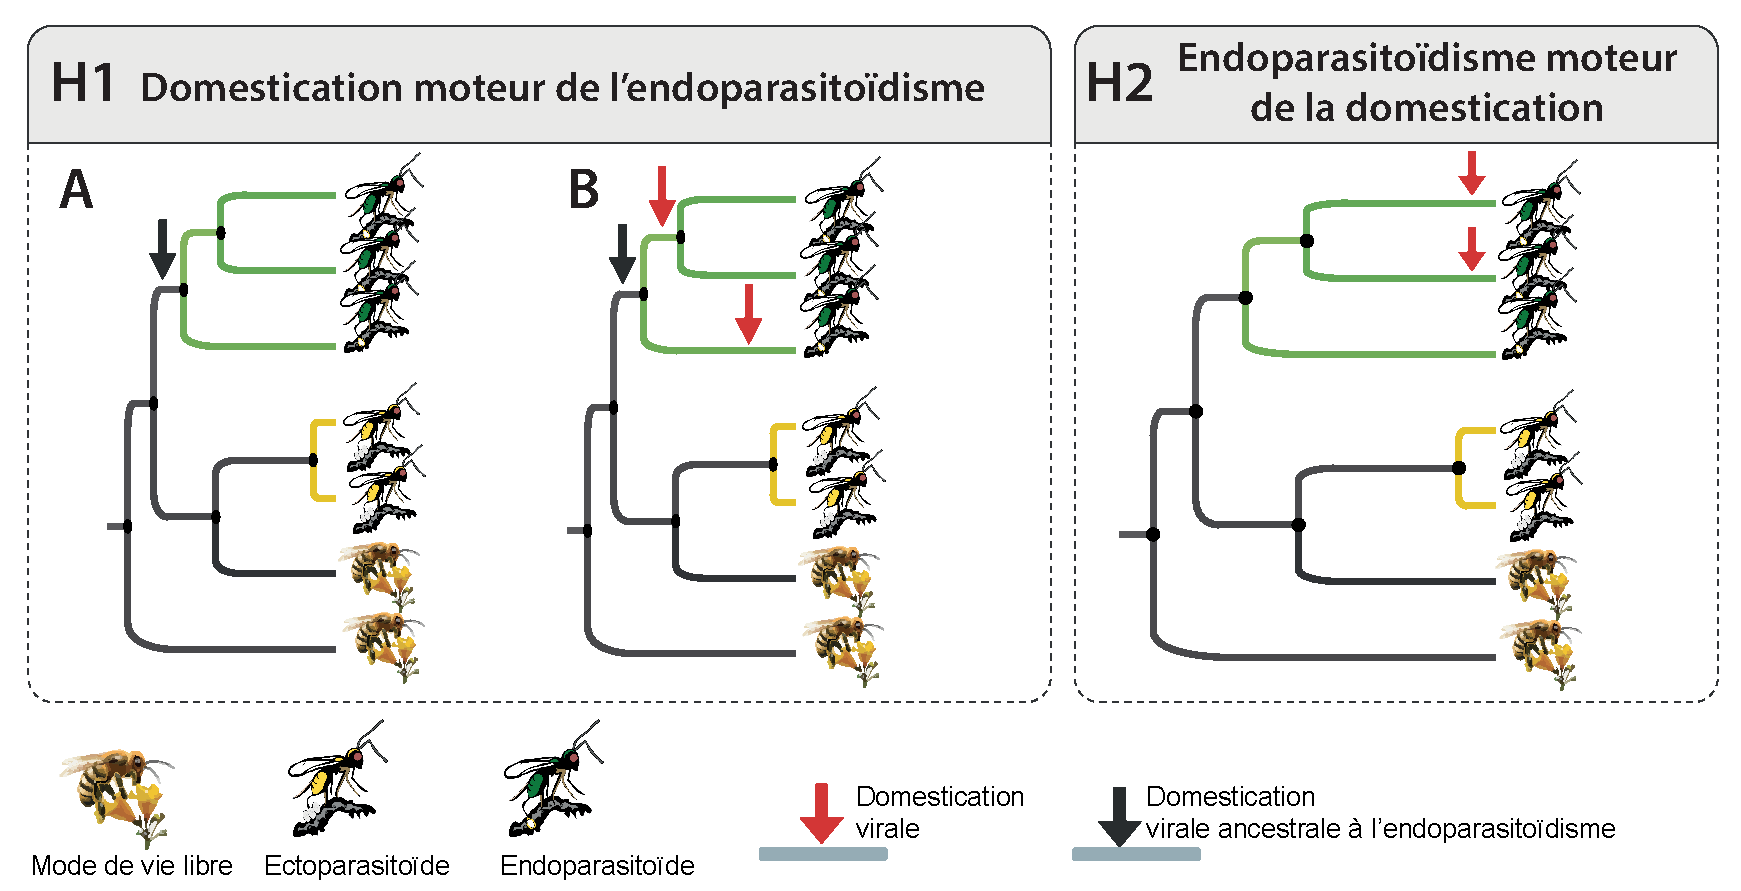
\includegraphics[width=\linewidth,height=\textheight,keepaspectratio]{PhD-master/figures/Endo_moteur_domestication.pdf}
\label{figure:Endo_moteur_domestication}
\end{figure}

Nous pourrions alors envisager ces deux hypothèses comme suit : \\

\textbf{Hypothèse 1}

Sous cette hypothèse, l'endogénisation et la domestication virale serait à l'origine de l'évolution de l'endoparasitoidisme. Cette hypothèse  peut être elle-même scindée en deux sous-hypothèses. La première (H1-A) impliquerait un évènement unique et ancestral de domestication ayant fortement favorisé l'apparition du mode de vie endoparasitoïde. La deuxième (H1-B) impliquerait également un évènement ancestral de domestication qui aurait été suivie de nombreux remplacements, à l'instar des syncitines chez les mammifères placentaire \citep{lavialle_paleovirology_2013}.\\ 

\textbf{Hypothèse 2}

Dans l'hypothèse alternative (H2), nous envisageons que l'évolution vers l'endoparasitoidisme n'implique pas de domestication virale, mais que plusieurs évènements de domestications, postérieurs à l'apparition du style de vie endoparasitoïde se seraient produits dans certaines lignées. Dans ce cas, ce serait le style de vie endoparasitoïde qui aurait favorisé la domestication de virus, via un avantage lié au contournement immunitaire. \\

Nous pourrions donc résumer H1 à une hypothèse selon laquelle la domestication aurait été un moteur de l'endoparasitoïdisme, alors que H2 serait l'hypothèse selon laquelle l'endoparasitoïdisme déjà bien établi, aurait été un moteur de la domestication.


\subsection{Évaluation de l'hypothèse H1}

Dans un premier temps, nous pouvons rechercher des arguments en faveur de la première hypothèse d'un seul évènement ancestral à l'endoparasitoïdisme (H1). Effectivement, dans nos données, nous observons plus d'évènements de domestication de virus dsDNA chez les endoparasitoïdes. Nous pourrions donc imaginer que toutes ces séquences proviennent d'un seul évènement ancestral. Seulement, ce n'est clairement pas le cas, car les gènes domestiqués ne présentent pas de signal phylogénétique dans ce sens, mais traduisent plutôt des évènements d'acquisitions indépendants. Ces données ne collent donc pas avec l'hypothèse (H1-A). En  revanche, l'hypothèse (H1-B) selon laquelle un évènement ancestral, suivi de plusieurs évènements de remplacements, serait envisageable.  Nous pourrions alors assister, comme chez les mammifères placentaires \citep{lavialle_paleovirology_2013}, à plusieurs événements récurrents de remplacements d'éléments viraux au cours de l'évolution, en gardant l'hypothèse d'une insertion ancestrale à l'origine de ce style de vie, mais qui en vue des remplacements, serait aujourd'hui impossible à détecter sur plus de 200 millions d'années d'évolution. De futures recherches pourraient supporter cette hypothèse en analysant, par exemple, les génomes d'autres espèces qui ont indépendamment évolué vers un mode de vie endoparasitoïde, comme les Diptères Tachinidae \citep{stireman_tachinidae_2006}. Sara Oukkal rédige d'ailleurs actuellement une partie de sa thèse sur ces points. 

Seulement, quelques espèces endoparasitoïdes de notre jeu de donnée ne présentaient pas d'évènement de domestication. En effet, dans le \hyperref[sec:chap1]{chapitre 1}, 3/37 des génomes endoparasitoïdes ne présentaient pas un seul EVE, et 15/37 endoparasitoïdes ne présentaient aucun évènement de domestication. Parmi ces parasitoïdes, certains ne presentaient dailleurs aucune trace de production de VLS. Par exemple, chez \textit{P. concolor} et \textit{P. lounsburyi}, aucun VLP ou PDVs n'a été détecté dans les glandes à venins et les ovaires des deux espèces \citep{mathe-hubert_comparative_2016}. Nous ne parvenons d'ailleurs pas à trouver de phénomène de domestication pour ces deux espèces. De plus, chez \textit{Eretmocerus}, les espèces étudiées ne présentent également pas de preuve de production de VLS \citep{gelman_host-parasite_2005}. Concernant \textit{Eretmocerus}, nous ne retrouvons d'ailleurs pas d'évènement de domestication de virus dsDNA. Nous pourrions ainsi imaginer, toujours sous l'hypothèse H1-B, qu'il y ait eu des pertes de ces fonctions virales chez ces espèces.


\subsection{Évaluation de l'hypothèse H2}

D'autres arguments font plutôt pencher la balance vers l'hypothèse (H2). 

\textbf{Pas de trace d'évènements aussi anciens que le clade des Parasitoida}\\
Le premier argument tient dans le fait que nous ne retrouvons aujourd'hui que des évènements postérieurs au groupe des Parasitoida. Par exemple, les plus anciens cas décrits à ce jour sont ceux des Microgastroïdes, il y a 100 millions d'années \citep{whitfield_virus_2003, bezier_bracovirus_2008, murphy_phylogeny_2008} et ceux découverts lors du \hyperref[sec:chap3]{chapitre 3} chez les Eucoilini, il y a 75 millions d'années. Cependant, ceci ne permet pas de rejeter complètement l'hypothèse H1-B impliquant des remplacements. \\

\textbf{Des stratégies n'impliquant pas de VLS endogénisés existent chez les endoparasitoïdes}\\
Chez de nombreuses espèces d'endoparasitoïdes, des stratégies d'inhibition du système immunitaire de l'hôte n'impliquant pas la production de VLS sont rencontrées. 
Par exemple, d'autres stratégies peuvent impliquer également des virus, mais non endogénisés. En effet, comme nous l'avons vu chez l'espèce \textit{Diachasmimorpha longicaudata}, il a pu être mis en évidence des effets protecteurs analogues aux polydnavirus et VLPs provenant d'un poxvirus mutualiste, sans pour autant présenter de domestication intra-génomique virus \citep{coffman_mutualistic_2020,coffman_viral_2022}, ou bien encore un ascovirus mutualiste (DpAV4) qui chez plusieurs espèces du genre \textit{Diadromus} permet lorsqu'il est injecté dans l'hôte, d'augmenter le succès du développement des progénitures \citep{stasiak_characteristics_2005}. Nous pourrions en revanche imaginer que ce sont ce genre d'interactions sur le long terme qui auraient participé à la rétention des gènes de ces virus mutualistes par ces guêpes au cours de l'évolution. \\

Enfin, chez certaines espèces endoparasitoïdes, le venin qui accompagne l'œuf est dépourvu de VLS \citep{moreau_venom_2015}. En effet, des espèces comme \textit{Pimpla hypochondriaca} et \textit{Pteromalus puparum} qui sont toutes des endoparasitoïdes de Lépidoptères, ou bien \textit{Aphidius ervi} qui est un endoparasitoïde de pucerons, présentent toutes des fonctions de contournement de l'immunité présent dans leur venin, sans pour autant produire de particules virales \citep{moreau_venom_2015}. Ceci constitue donc un contre-argument à l'hypothèse H1, car d'autres stratégies retrouvées chez des guêpes endoparasitoïdes existent sans présenter de trace de production de VLS. Néanmoins, nous pourrions envisager qu'il y ait eu, en particulier chez ces espèces, une perte secondaire de la production de VLS.\\ 

\textbf{Une "amélioration" de fonction apportée par la domestication chez les guêpes endoparasitoïdes?}\\
Nous pourrions formuler l'hypothèse que l'apport de la domestication virale aurait en quelque sorte "amélioré" le système pré-existant chez de nombreuses espèces endoparasitoïdes. Certains arguments vont en faveur de cette hypothèse. En effet, les venins d'endoparasitoïdes sont également impliqués dans des interactions synergiques avec les PDV/VLP dans certains systèmes hôte-endoparasitoïde \citep{asgari_venom_2006,asgari_venom_2011,schmidt_innate_2001}. Des études suggèrent que le venin renforce l'effet des PDVs. Par exemple chez \textit{Microplitis demolitor} sur les hémocytes de l'hôte (inhibition de l'étalement cellulaire) de manière dose-dépendante, et retarde également le développement de l'hôte \citep{strand_developmental_1991,strand_alterations_1991}. Le venin est également nécessaire pour l'entrée et le déballage des PDVs chez \textit{Cotesia melanoscela} \citep{stoltz_venom_1988}, et chez \textit{Cotesia rubecula}, les gènes de virulence ne sont même pas exprimés dans les hémocytes en l'absence de certains peptides présents dans le venin \citep{zhang_novel_2004} (voir \citep{moreau_venom_2015} pour revue). Par conséquent, étant donné que les systèmes VLS dépendent du venin injecté, il est probable que ces systèmes se sont adaptés à un système de production de venin existant qui ne comportait pas au préalable de VLS.\\

Enfin, certains des gènes ou protéines de virulence présents dans les polydnavirus et les VLPs sont dérivés des guêpes \citep{desjardins_comparative_2008,burke_systematic_2014, huguet_evolution_2012}, tandis que d'autres plus rares dérivent d'éléments transposables (TE) \citep{zhang_chromosome-level_2019, gauthier_chromosomal_2021}, et on imagine que ces gènes ont ensuite été transférés dans le provirus qui constituent \textit{in fine} les cercles d'ADN par exemple \citep{herniou_when_2013}. Ces gènes (ou leurs protéines codées) aujourd'hui présents dans les VLPs ou les PDVs étaient probablement déjà présents dans les génomes des guêpes avant la domestication et  rentraient déjà dans la composition du venin des guêpes ancestrales, participant ainsi à réguler le métabolisme et l'immunité de l'hôte. Les VLPs ou VLS auraient "simplement" constitué un moyen plus efficace pour délivrer ces facteurs de virulence aux cellules cibles. \\

\textbf{Conclusion sur cette partie}

Prises dans leur ensemble, ces observations tendent donc à favoriser la deuxième hypothèse (H2) selon laquelle l'endoparasitoïdisme ne serait pas né d'une domestication ancestrale, mais que plusieurs évènements de domestications seraient apparus indépendamment le long de la phylogénie des Hyménoptères, sans que tous les clades ne soient concernés. Et ceci se serait produit particulièrement au sein des clades endoparasitoïdes dont le style de vie aurait favorisé la rétention de ces gènes viraux à des fins d'adaptation face au système immunitaire de leurs hôtes.  


\section{La domestication comme moteur du succès évolutif}

Sur le plan évolutif, ces évènements de domestication ont probablement chamboulé la trajectoire évolutive des espèces concernées dont les descendants représentent aujourd'hui une grande diversité d'espèces. Le groupe des microgastroïde est un bon exemple. Il s'agit de l'ensemble des espèces dont l'ancêtre commun a vraisemblablement acquis puis domestiqués une batterie de gènes provenant d'un nudivirus ancestral il y a 100 millions d'années \citep{murphy_phylogeny_2008, whitfield_estimating_2002,banks_dissecting_2006}. Aujourd'hui, ce groupe représente une partie importante de la diversité des Ichneumonoidea avec 46,000 espèces estimées dans le monde \citep{rodriguez_extrapolations_2013}. 
Ces résultats suggèrent donc que sur de longues périodes, la domestication virale a contribué activement à la radiation du clade.\\
De la même manière, nous avons observé dans le \hyperref[sec:chap3]{chapitre 3} qu'une domestication virale ancienne chez l'ancêtre commun du clade diversifié des Eucoilini pourrait avoir eu des conséquences très importantes dans l'évolution de ce clade via la production de VLPs que nous observons chez au moins 2 genres de ce groupe. \\

\section{Domestication de virus filamenteux chez les Eucoilini}

En ce qui concerne les Eucoilini, nous avons pu identifier deux cas distincts d'endogénisation. Le premier cas concerne un pool de 18 gènes domestiqués chez presque toutes les espèces d'Eucoilini étudiées, dont l'ancêtre commun aurait acquis ces gènes il y a environ 75 millions d'années \citep{blaimer_comprehensive_2020}. Le second cas, plus récent, concerne un pool de 9 gènes provenant d'un seul membre de ce groupe dans le genre \textit{Rhoptromeris}. Dans les deux cas, les génomes viraux endogénisés provenaient de virus filamenteux, LhFV étant le plus étroitement lié au premier événement et LbFV au second (\figurename{\ref{figure:Microscopie_trybliographa}}).

\begin{figure}[!htpbt]
\captionsetup{font=footnotesize}
 \centering
  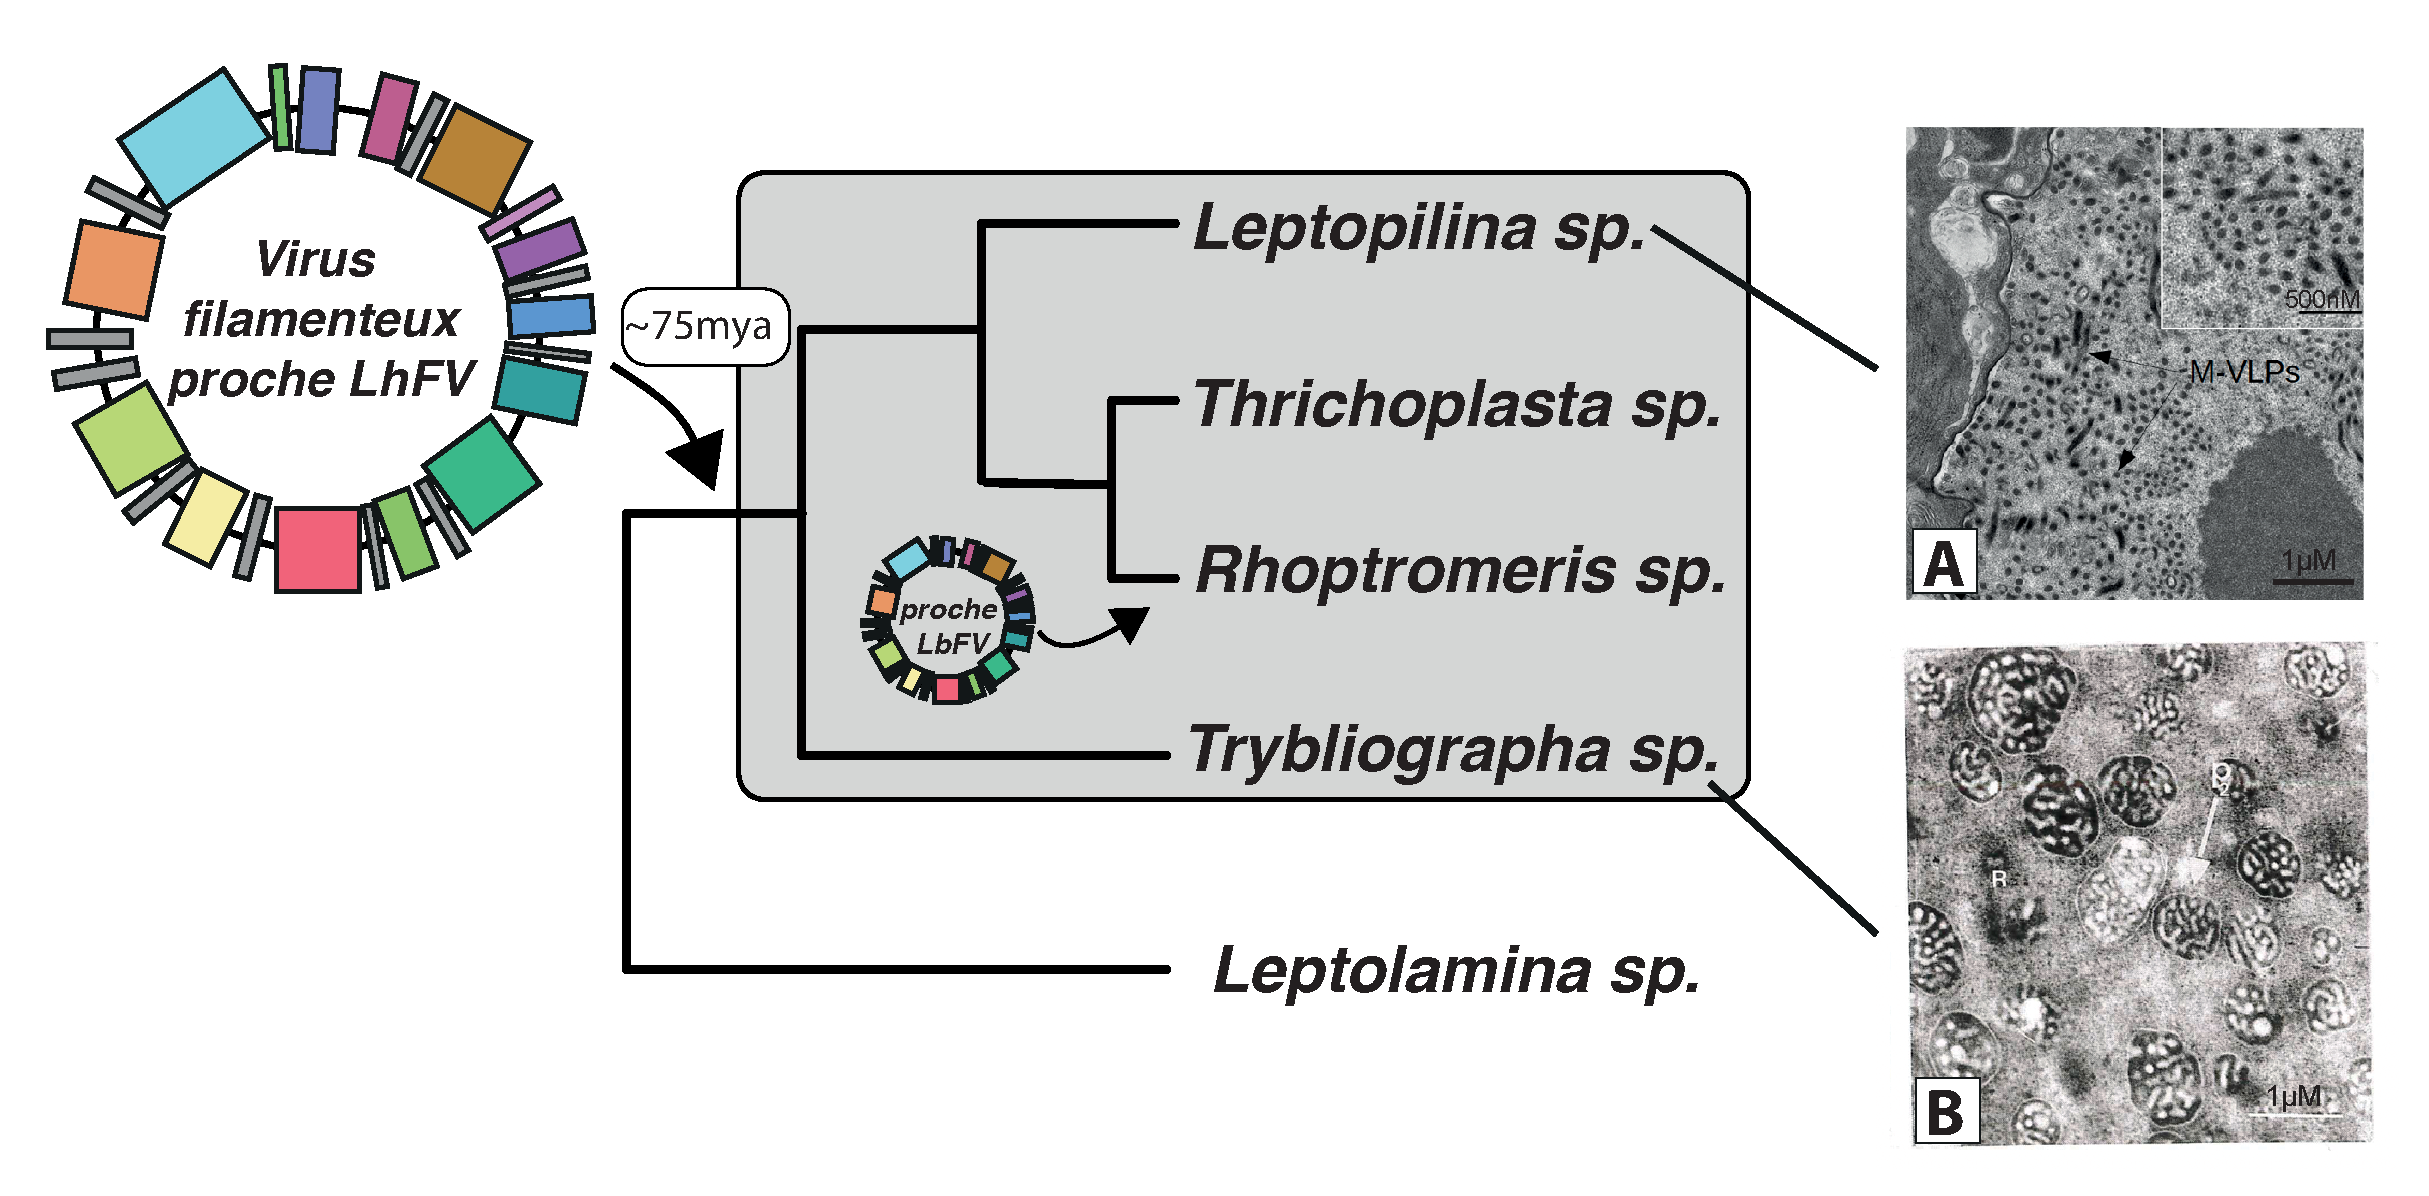
\includegraphics[width=\linewidth,height=\textheight,keepaspectratio]{PhD-master/figures/Microscopie_trybliographa.pdf}
\caption[Discuss:Résumé graphique des deux évènements indépendants d'endogénisations chez les Eucoilini]{\textbf{Résumé graphique des deux évènements indépendants d'endogénisations chez les Eucoilini}. VLPs produits dans la glande à venin de \textit{Lepoptilina boulardi} (A) et \textit{Trybliographa rapae} (B)  photos de (Di Giovanni et al., 2020) et D.Poinçot et K.Haddj E PhD 1999.}
\label{figure:Microscopie_trybliographa}
\end{figure}

Il est clair que les 18 EVEs de l'événement initial jouent un rôle dans le développement des VLPs. 13 de ces 18 EVEs sont spécifiquement exprimées dans la glande à venin au début du stade nymphal de la guêpe, lorsque les VLPs sont synthétisées, comme décrit dans \cite{di_giovanni_behavior-manipulating_2020}. Par conséquent, nous nous attendons à ce que les cinq EVEs supplémentaires retrouvés dans notre analyse au \hyperref[sec:chap3]{chapitre 3} présantent les mêmes profils d'expression. Par ailleurs, comme on pourrait s'y attendre pour des gènes impliqués dans la production de VLPs, nous observons des signaux extrêmement forts de sélection purificatrice pour tous les EVEs provenant de l'événement d'endogénisation initial, y compris pour les 5 nouveaux (\figurename{\ref{figure:Cynipids_VLPS_updated_discuss}}-1).\\ 

Concernant les fonctions de ces EVEs, nous retrouvons les gènes \textit{lef-4}, \textit{lef-9} et \textit{lef-8} chez toutes les espèces concernées par l'évènement ancestral chez les Eucoilini. Avec le facteur d'initiation (\textit{lef-5}) identifié par mon analyse, ceci suggère que toutes ces guêpes possèdent les gènes nécessaires pour former un complexe complet d'ARN polymérase (\figurename{\ref{figure:Cynipids_VLPS_updated_discuss}}-3). De plus, la présence d'une \textit{helicase} et \textit{ADN polymerase} filamenteuses suggère qu'une partie de la machinerie ancestrale de réplication de l'ADN viral est encore fonctionnelle chez les espèces Eucoilini (\figurename{\ref{figure:Cynipids_VLPS_updated_discuss}}-2). En effet, il a été démontré que dans ce système, 10 des 13 EVEs sont amplifiés chez ces guêpes (Di Giovanni et al., 2020). L'hypothèse la plus vraisemblable étant que c'est l'ADN polymérase du virus filamenteux (ORF58) qui permet cette amplification qui augmenterait donc leur profil d'expression des EVEs (Di Giovanni et al., 2020). Plusieurs gènes sont également probablement impliqués dans l'enveloppement des protéines de virulence (\textit{ac81}), le développement des membranes lipidiques (\textit{lcat}), et éventuellement l'entrée des composants viraux dans les cellules hôtes par liaison à des récepteurs de surface cellulaire (\textit{LhFV contig223 orf23}) (\figurename{\ref{figure:Cynipids_VLPS_updated_discuss}}-4). Ce dernier gène (LhFV contig223 orf23) est présent chez tous les Eucoilini, mais chez \textit{Rhoptromeris}, il est probablement le résultat d'un remplacement suite au deuxième événement d'endogénisation. Par conséquent, il est possible que l'apparition d'une deuxième copie homologue de cette protéine à ce moment ait été fortement sélectionnée, car elle aurait conféré un avantage (\figurename{\ref{figure:Cynipids_VLPS_updated_discuss}}-4).\\

\begin{figure}[!htpbt]
\captionsetup{font=footnotesize}
 \centering
  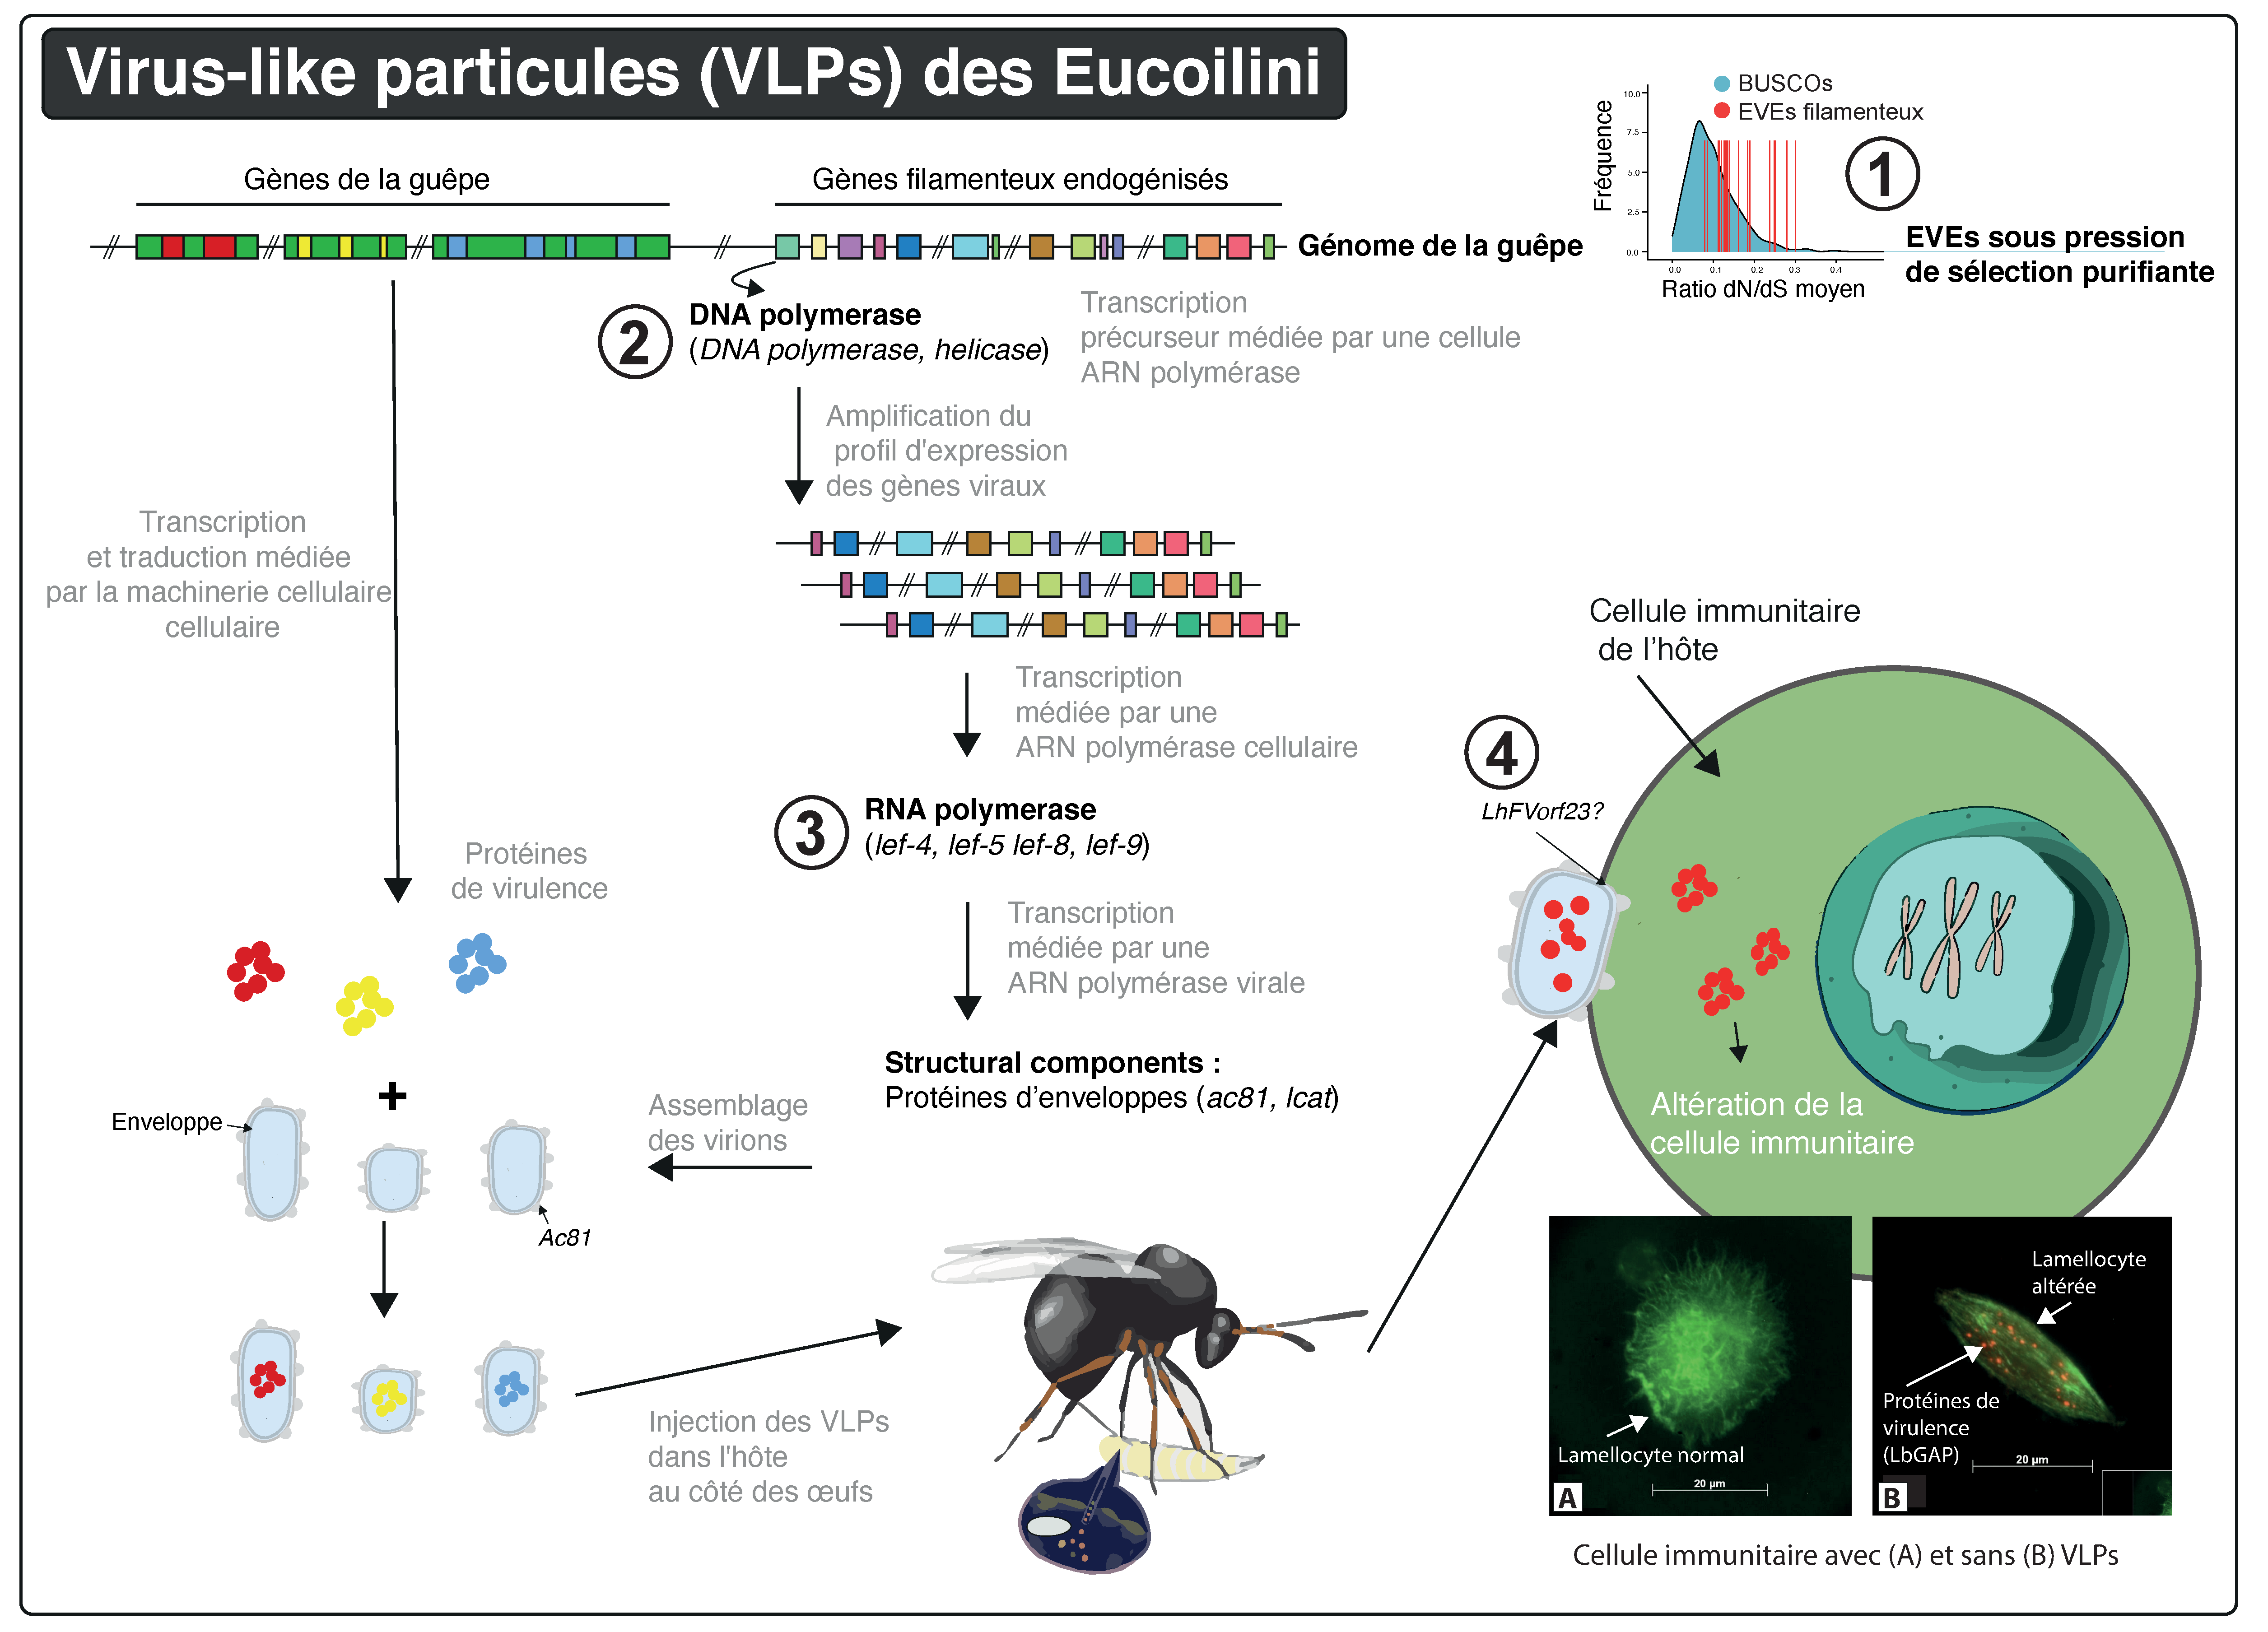
\includegraphics[width=\linewidth,height=\textheight,keepaspectratio]{PhD-master/figures/Cynipids_VLPS_updated_discuss.pdf}
\caption[Discuss:Résumé graphique putatif de la machinerie virale filamenteuse produisant des VLPs chez les Eucoilini]{\textbf{Résumé graphique putatif de la machinerie virale filamenteuse produisant des VLPs chez les Eucoilini}.}
\label{figure:Cynipids_VLPS_updated_discuss}
\end{figure}

Finalement, sur la base de l'ensemble de ces données, nous disposons de suffisamment d'éléments pour conclure que chez ces Eucoilini, les EVEs d'origine filamenteux sont très probablement impliqués dans la formation des VLPs. Dans le cas contraire où seuls certaines espèces de ce groupe auraient usage de ces VLPs, nous nous attendrions à ce que les 18 EVEs chez ces espèces ait dégénéré, or, tous ces gènes sont intacts après plus de 75 millions d'années d'évolution. De plus, la présence de VLPs dans les glandes à venin de l'espèce \textit{Trybliographa rapae} la plus basale du groupe Eucoilini concernée par l'événement, renforce cette hypothèse (thèse de Nabila Kacem Haddj El Mrabet en 1999) (\figurename{\ref{figure:Microscopie_trybliographa}}).\\ 

À la lumière de ces résultats, nous pourrions supposer que, tout comme les Microgastroïdes et leurs polydnavirus, la production de VLPs par les Eucoilini aurait également contribué au succès écologique et à la radiation du groupe. En effet, parmi les Figitidae, qui comportent près de 140 genres pour 1,569 espèces de guêpes, la sous-famille des Eucoilinae est de loin la plus riche en espèces avec plus de 80 genres et plus de 900 espèces décrites, soit près de 33\% de la diversité des Figitidae \citep{ronquist_phylogeny_1995}. Connaitre la diversité spécifique que représente les Eucoilini dans tout ça en revanche est plus difficile. Mais par exemple, le complexe "\textit{Eucoila}/\textit{Trybliographa}" au sein de cette tribu est l'un des groupes d'eucoilines les plus communs et les plus riches en espèces dans l'hémisphère nord (thèse de Mattias Forshage). \\

Par ailleurs, d'autres éléments pourraient nous faire penser que cet évènement de domestication a participé au succès évolutif de ce groupe. En effet, les résultats du \hyperref[sec:chap2]{chapitre 2} permettent d'estimer l'âge de l'évènement d'endogénisation virale entre 55 et 100 millions d'années, ce qui correspond à peu près à la période durant laquelle les hôtes Diptères (Schizophora) des Eucoilini ont commencé à se diversifier (entre 55 et 60 millions d'années) \citep{wiegmann_episodic_2011}. Ainsi, nous pourrions avancer que cette innovation génétique soudaine aurait permis à ces guêpes de coloniser et de s'adapter à leurs hôtes Schizophora au cours de la radiation du groupe.\\

Pour que ces deux événements d'endogénisation aient pu se produire indépendamment dans la lignée des Eucoilini (\hyperref[sec:chap3]{chapitre 3}) et plus généralement chez de nombreuses autres espèces endoparasitoïdes (\hyperref[sec:chap2]{chapitre 2}), il doit y avoir eu une longue période d'interaction étroite entre les Filamentoviridae et les guêpes. Dans la partie suivante, je discuterai les particularités de cette relation. 

\section{Les Filamentoviridae}

\subsection{Filamentoviridae : Préférence pour les endoparasitoïdes?}

Tous les Filamentoviridae analysés dans le \hyperref[sec:chap2]{chapitre 2} ont été découverts chez des guêpes endoparasitoïdes (\figurename{\ref{figure:Heatmap_NCBI4}}-A), cependant, pour éviter les biais inhérents aux thèmes de recherche de nos deux équipes, qui se sont surtout concentrées sur les endoparasitoïdes, nous avons recherché de manière systématique la présence d'éléments génétiques filamenteux dans des bases de données publiques (NBCI et BIPPA). Et ceci, en incluant tous les génomes d'Hyménoptères, mais également des hôtes putatifs des guêpes que sont les Lépidoptères et les Diptères. Ainsi, l'analyse systématique de 2815 génomes (couvrant 1576 espèces) n'a trouvé aucune preuve de la présence de génome de Filamentoviridae sauf chez des espèces endoparasitoïdes (9 au total si nous incluons tous les filamenteux connus). (\figurename{\ref{figure:Heatmap_NCBI4}}-B). \\

\textbf{Distribution intra-Hyménoptères}

Plus spécifiquement, au sein des Hyménoptères, les virus filamenteux semblent se répliquer préférentiellement chez les espèces endoparasitoïdes, puisque 40 des 87 génomes endoparasitoïdes analysés contenaient des EVEs contre seulement 3 des 209 Hyménoptères vivant librement et 0 des 29 ectoparasitoïdes. Aussi, il semblerait qu'à l'échelle des Hyménoptères, les virus filamenteux se soient spécifiquement adaptés aux Hyménoptères présentant un mode de vie endoparasitoïde, dont elles tirent, peut-être, profit. En effet, ce mode de vie pourrait représenter une niche écologique favorisant le maintien et la propagation de ces virus au sein des populations de guêpes, à la fois verticalement de la mère à la progéniture \citep{martinez_additional_2016, coffman_viral_2022} et horizontalement entre parasitoïdes non apparentés partageant le même hôte \citep{varaldi_infectious_2003,stasiak_characteristics_2005}.\\

Nos analyses de datation de la famille en \hyperref[sec:chap3]{chapitre 3} apportent également des éléments pour alimenter ces réflexions. Ces analyses ont révélé que les Filamentoviridae auraient divergé il y a entre 233 à 370 millions d'années (\figurename{\ref{figure:Cynipoidea_dsDNA_datation_plot}}), ce qui coïncide avec la période où les Hyménoptères ont commencé à se diversifier entre le Carbonifère et le Trias (239-329 millions d'années) \citep{peters_evolutionary_2017}. Ces données donnent à penser que l'origine de ces virus est sensiblement plus ancienne que celle du principal clade de guêpes parasitoïdes (les "parasitoida") qui ont divergé entre 195 et 266 millions d'années. Nous pourrions donc imaginer que les ancêtres filamenteux se seraient d'abord développés en infectant les premiers Hyménoptères avant de se spécialiser sur des Hyménoptères au style de vie endoparasitoïdes.\\

\textbf{Distribution chez les hôtes des parasitoïdes}

Nous retrouvons également la présence de gènes filamenteux dans les génomes de Diptères et de Lépidoptères, mais en bien plus faible fréquence que chez les Hyménoptères (\figurename{\ref{figure:Heatmap_NCBI4}}-A et B). Ces deux ordres non Hyménoptère sont des hôtes privilégiés pour de nombreux Hyménoptères parasitoides. Ces insertions peuvent provenir d'infections filamenteuses passées ou en cours. De manière intéressante, une étude antérieure a mis en évidence des virus filamenteux se reproduisant chez les lépidoptères \citep{styer_new_1987}. Cependant, puisqu'aucune donnée de séquence n'est disponible pour ces virus, nous ne pouvons pas affirmer qu'ils appartiennent à la famille des Filamentoviridae. Dans nos données, nous ne retrouvons aucun signe d'infection en cours. En effet, en cas d'infection, on s'attendait à retrouver la plupart des gènes cœurs dans les scaffolds séquencés. Au contraire, nous n'avons retrouvé que quelques gènes, qui, de plus, se retrouvent pour la plupart dans des scaffolds trop grands pour correspondre à un génome viral. 

Bien que les données n'apportent pas de preuve de l'existence de lignées de Filamentoviridae infectant les Lépidoptères ou les Diptères, nous ne pouvons pas exclure qu'une partie inconnue de la diversité des Filamentorividae se soit spécialisée chez les Lépidoptères, voire les Diptères.\\

\textbf{Perspective de travail sur cette partie}

En perspective de ces travaux, afin d'expliquer davantage cette préférence pour les endoparasitoïdes, nous pourrions envisager d'étendre notre recherche systématique de virus filamenteux à l'échelle des données brutes SRA. En effet, nous pourrions imaginer que les auteur.ices.s des génomes assemblés aient arbitrairement supprimé tout scaffold dérivé d'un virus, nous empêchant ainsi de constater la présence de scaffolds filamenteux libres chez les espèces non endoparasitoïdes. Cependant, il n'y a aucune raison de croire que ce processus ne soit envisagé que pour les génomes des Lépidoptères et des Diptères et non pour les Hyménoptères endoparasitoïdes. De plus, ces analyses mériteraient d'être poursuivies en recherchant sur une plus large gamme d'organismes la présence de virus filamenteux exogènes ou endogènes afin de vérifier si seuls ces insectes sont concernés. Dans le cas d'une préférence pour le mode de vie endoparasitoïde, il n'y a aucune raison de penser que des traces de virus filamenteux seraient présents chez des espèces qui n'interagissent pas avec ce mode de vie. Enfin, nous avons l'intention d'étudier plus précisément l'effet du mode de vie endoparasitoïde sur l'existence de ces virus en intégrant l'inertie phylogénétique, qui n'est pas encore prise en compte dans nos recherches, car elle nécessite d'obtenir une phylogénie complète des espèces analysées. \newpage


\subsection{Filamentoviridae : Une source d'innovation génétique ?}

\begin{figure}[H]
\captionsetup{font=footnotesize}
 \centering
  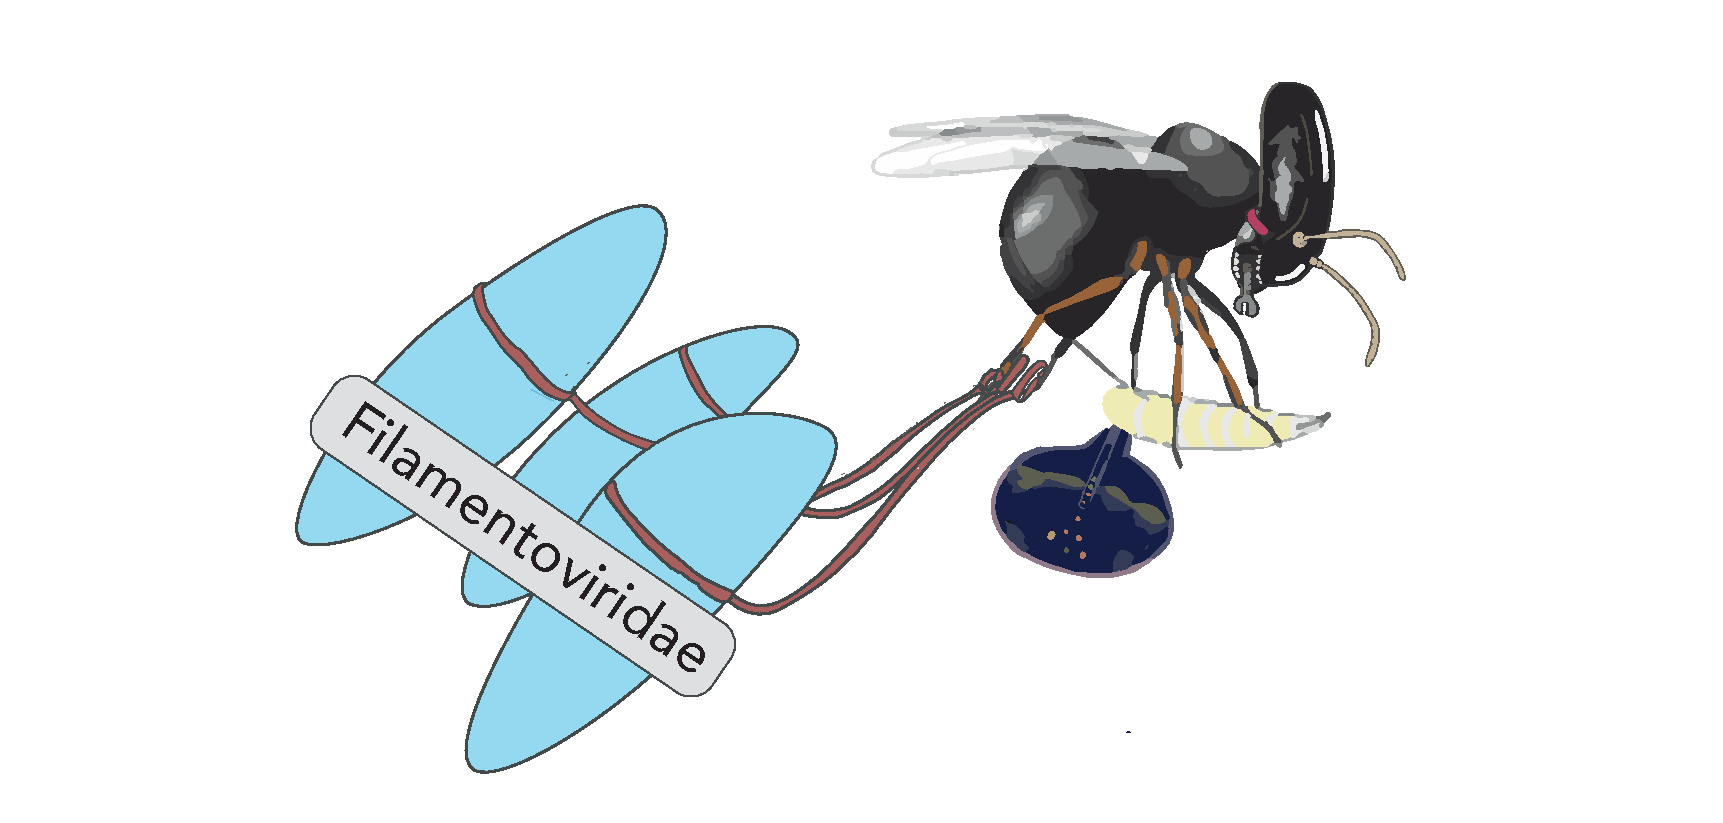
\includegraphics[width=\linewidth,height=\textheight,keepaspectratio]{PhD-master/figures/Domestication_illustration_Eucoilini.pdf}
\label{figure:Domestication_illustration_Eucoilini}
\end{figure}

\textbf{Du côté des guêpes}

Au moins deux fois par le passé, il y a 75 millions d'années chez les Eucoilini et plus récemment chez une espèce de Platygastroidea (\textit{P.orseoliae}), nous avons montré que l'insertion de virus filamenteux a pu entraîner une domestication moléculaire. Dans le premier scénario présenté, la fonction est orientée vers la synthèse de VLPs impliqués dans la protection de la progéniture contre le système immunitaire de l'hôte. Dans le second scénario, plus récent, cela est moins évident et il faudrait des preuves supplémentaires, comme la transcriptomique et la microscopie électronique, pour tester nos hypothèses selon lesquels les ORFs filamenteux sont à l'origine de la production de VLPs. D'autres cas d'endogénisation ont également été proposés sans révéler de preuve de domestication comme chez \textit{Dolichomitus} \citep{burke_endogenization_2020}, ou bien plusieurs espèces d'Hyménoptères, Diptères et Lépidoptères dans les \hyperref[sec:chap1]{chapitre 1} et \hyperref[sec:chap2]{chapitre 2}.\\

Aussi, il apparait que les phénomènes de domestication tels qu'envisagés lors de la production de structures virales sont encore rares du côté des virus filamenteux. Néanmoins, nous montrons tout de même dans les \hyperref[sec:chap1]{chapitre 1} et \hyperref[sec:chap2]{chapitre 2} plusieurs cas d'insertions filamenteux potentiellement adaptatives et l'étude de ces insertions serait nécessaire pour connaitre leurs fonctions spécifiques. Ainsi, si ces relations filamenteux-endoparasitoïdes existent, nous devrions, en continuant à séquencer les endoparasitoïdes, trouver de plus en plus d'exemples de domestication de ce type. \\

\newpage

\textbf{Du côté des hôtes des guêpes}

Nous venons d'aborder l'aspect endoparasitoïde, mais nous pouvons également discuter de la nature adaptative des insertions filamenteuses chez les hôtes des guêpes parasitoïdes.

Parmi les Diptères et les Lépidoptères, deux ordres attaqués par les guêpes endoparasitoïdes, nous avons constaté dans le \hyperref[sec:chap2]{chapitre 2} que la majeure partie de ces EVEs filamenteux étaient dégradés, ce qui suggère qu'il s'agit d'insertions plutôt anciennes et non fonctionnelles (\figurename{\ref{figure:Heatmap_NCBI4}}-B). Quelques-uns de ces gènes sont en revanche toujours intacts et pourraient toujours êtres fonctionnels dans le génome de certains Diptères ou Lépidoptères. Ces gènes encore intacts pourraient provenir d'insertions trop récentes pour voir l'apparition de codons stop prématurés suite à une pseudogénisation. Néanmoins, dans la littérature, des études ont déjà montré que les guêpes parasitoïdes et leurs hôtes subissent des transferts de gènes médiés par des virus endogènes \citep{muller_investigating_2022, gasmi_recurrent_2015,di_lelio_evolution_2019}. Par exemple, un THG d'un gène de guêpe, "\textit{Sl gasmin}", surement médié par un polydnavirus (PDVs), joue un rôle central dans la médiation de la phagocytose bactérienne dans les hémocytes de papillon de nuit \textit{Spodoptera littoralis} \citep{di_lelio_evolution_2019}. Nous pourrions donc imaginer que chez les espèces présentant des PDVs et des virus filamenteux, des transferts de gènes aient été médiés de la même façon des génomes filamenteux vers les génomes des Lépidoptères. D'autres exemples montrent également des THG d'une famille de protéines toxiques virales appelées parasitoid killing factor (PKF). Dans ce cas, ces facteurs sont retrouvés dans les génomes des virus présent chez les Lépidoptères (entomopoxvirus, ascovirus, et baculovirus). Certaines espèces de lépidoptères auraient acquis des PKF provenant de ces virus, et ceux-ci fournissent des armes spécifiques qui permettent de contrer les attaques de certains parasitoïdes en particulier \citep{gasmi_horizontally_2021}.\\ 

Ces deux exemples laissent entrevoir des routes de transmission potentielles entre les virus filamenteux et les Lépidoptères, soit via l'interaction hôte-parasitoïde (médié possiblement par des PDVs), soit via l'interaction directe entre Filamenteux-Lépidoptères.

De manière intéressante, certains EVEs filamenteux sont présents chez plusieurs espèces de Lépidoptères du même genre, ce qui suggère que leur endogénisation pourrait avoir eu lieu chez leur ancêtre commun. En effet, par exemple chez 4 espèces du genre \textit{Apodemia} présentant des homologies de séquence avec LbFVorf20, on retrouve effectivement une phylogénie du gène qui place ces séquences dans un groupe monophylétique. De même par exemple dans le cas du gène \textit{pif-5} retrouvé chez 3 espèces du genre \textit{Junonia}. Cependant, à regarder les phylogénies des gènes, on se rend compte que ces séquences forment un râteau, ce qui est peu probable sous l'hypothèse d'une endogénisation chez l'ancêtre commun de ces deux genres, car nous devrions observer des différences le long des séquences (\figurename{\ref{figure:Host_filamentous_EVES_phylogeny}}).\\

Une hypothèse que nous pourrions formuler concernant l'acquisition de ces gènes pourrait être celle d'un transfert médié par des baculovirus de Lépidoptères. Ce genre de cas a déjà été décrit dans la littérature. En effet, \cite{gilbert_continuous_2016} ont par exemple pu montrer, en analysant les génomes de plusieurs populations de baculovirus infectieux de Lépidoptères, des transferts d'éléments transposables et d'autres séquences provenant des Lépidoptères vers les génomes des baculovirus (4.8\% des génomes viraux séquencés portaient au moins une insertion). Cette étude a ensuite fournit également des arguments suggérant l'implication des baculovirus en tant que vecteurs de transfert horizontal entre lépidoptères (voir aussi \citep{keeling_functional_2009,jehle_horizontal_1998,gilbert_population_2014}). En ce qui concerne les 2 gènes évoqués précédemment, nous pourrions imaginer que les Lépidoptères puissent être infectés par une lignée de virus filamenteux qui interagirait avec les baculovirus dans les cellules de ces insectes. Lors de ces interactions, des échanges génétiques auraient pu avoir lieu entre les filamenteux et les baculovirus. Certains ET Lépidoptères présents dans les génomes de baculovirus auraient ainsi pu médier un transfert de ces gènes filamenteux dans un second temps entre espèces  de Lépidoptères. Ce qui pourrait expliquer ce fameux râteau dans la phylogénie. Nous pourrions également imaginer que les génomes de virus filamenteux agissent même sans l'intermédiaire des baculovirus, et soient également des vecteurs de transfert horizontaux. Bien évidemment, pour confirmer ou non ces hypothèses, de nombreuses analyses seraient nécessaires, comme vérifier la présence d'évènements de transpositions dans les séquences flanquants ces gènes, ou bien vérifier que le long des génomes de baculovirus, nous trouvions effectivement des gènes filamenteux. 

\begin{figure}[!htpbt]
\captionsetup{font=footnotesize}
 \centering
  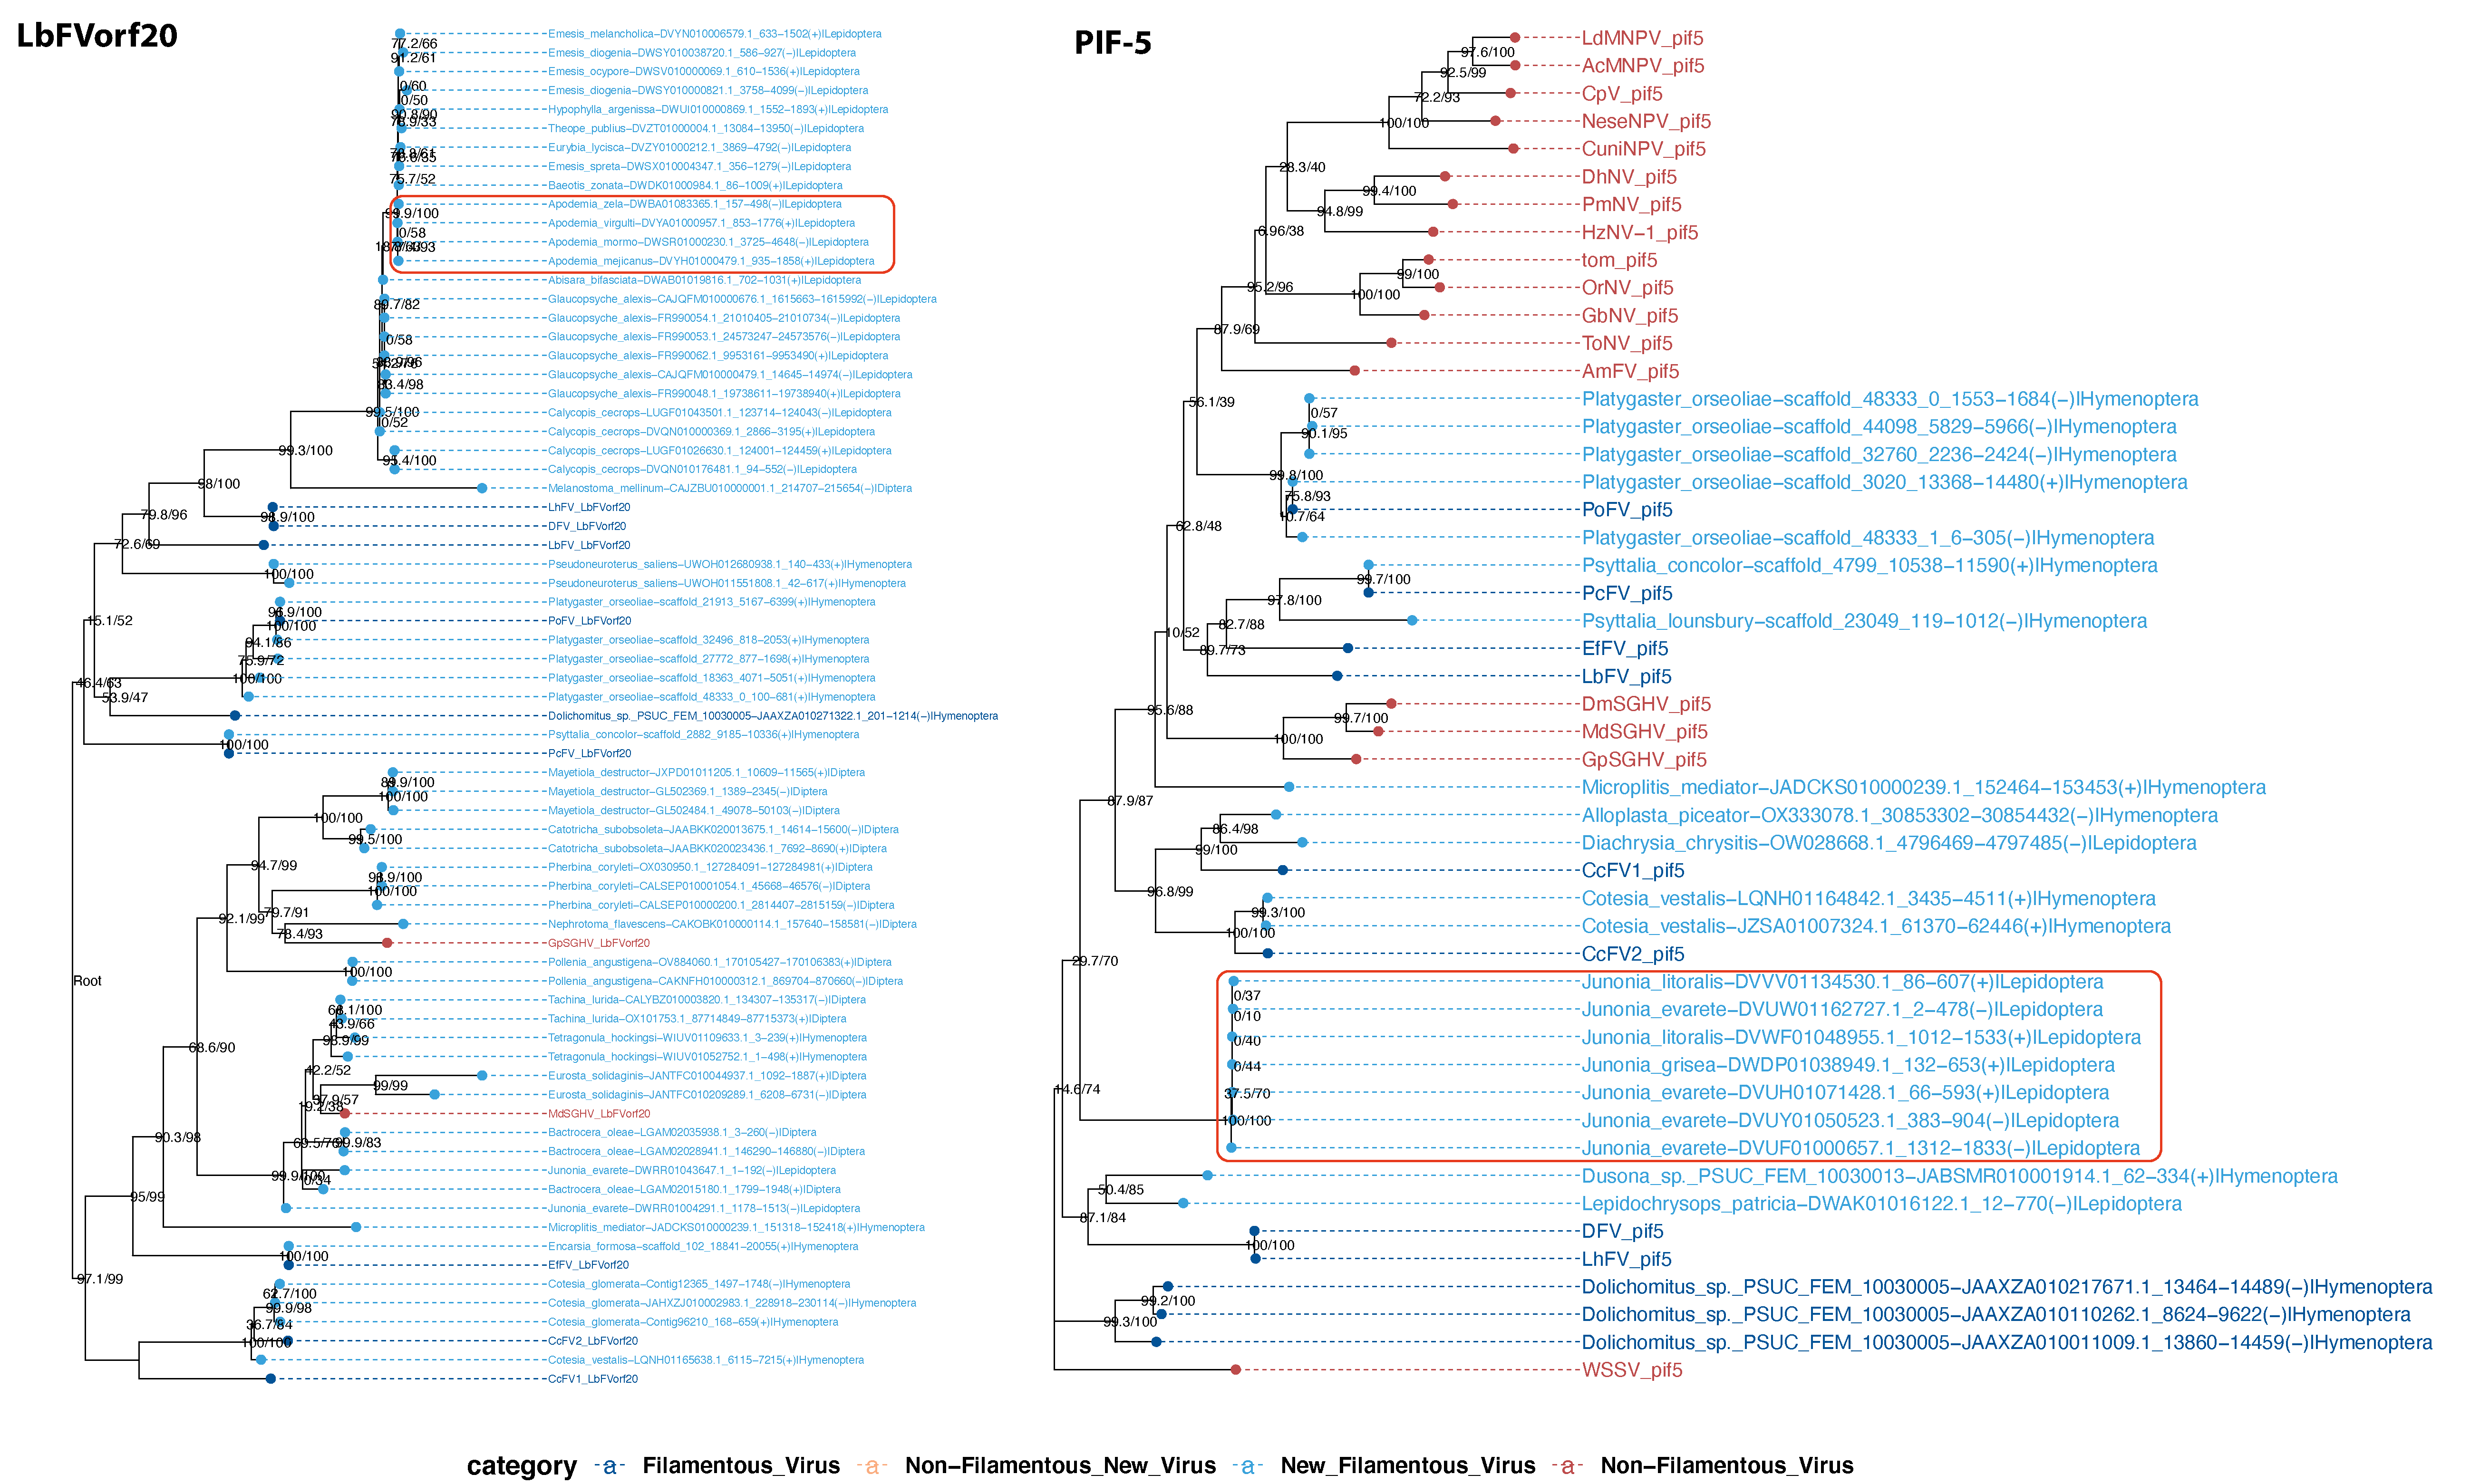
\includegraphics[width=\linewidth,height=\textheight,keepaspectratio]{PhD-master/figures/Host_filamentous_EVES_phylogeny.pdf}
\caption[Discuss:Phylogénies des gènes filamenteux LbFVorf20 et pif-5]{\textbf{Phylogénies des gènes filamenteux LbFVorf20 et pif-5}. Ces phylogénies comportent des séquences de virus filamenteux (bleu foncé), d'autres virus (rouge), et d'EVEs chez des espèces d'insectes dont l'ordre est indiqué après le pipe sur chaque séquence (bleu clair). Les figures d'alignements protéiques de ces deux gènes, comprenant uniquement les espèces du genre \textit{Glaucopsyche} et \textit{Apodemia} avec toutes les séquences virales, sont disponibles via les liens GitHub suivants : \href{https://github.com/BenjaminGuinet/PhD_defense/blob/main/Discussion/LbFVorf20_lepido_filamentous_MSA.pdf}{LbFVorf20} et \href{https://github.com/BenjaminGuinet/PhD_defense/blob/main/Discussion/Pif5_lepido_filamentous_MSA.pdf}{Pif5}.}
\label{figure:Host_filamentous_EVES_phylogeny}
\end{figure}


\newpage

\subsection{Filamentoviridae : Manipulation du comportement de ponte, une caractéristique de la famille?}

\begin{figure}[H]
\captionsetup{font=footnotesize}
 \centering
  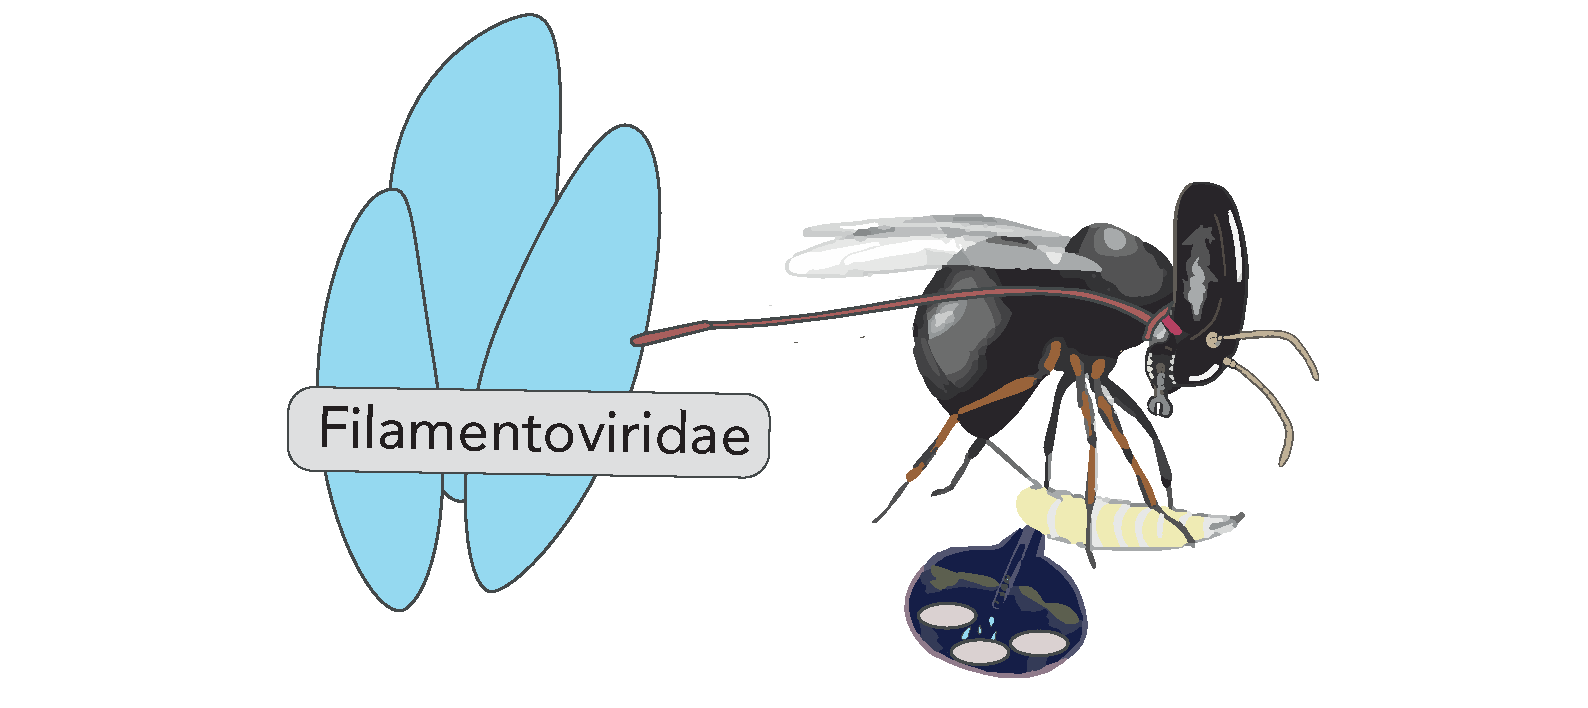
\includegraphics[width=\linewidth,height=\textheight,keepaspectratio]{PhD-master/figures/Manipulation_illustration_Eucoilini.pdf}
\label{figure:Manipulation_illustration_Eucoilini}
\end{figure}

LbFV qui fait partie de la famille des Filamentoviridae a un fort impact sur le comportement de ponte de son hôte \textit{L.boulardi}. Dans ce cas, les femelles infectées par LbFV acceptent facilement de pondre leurs œufs dans des hôtes déjà parasités, contrairement aux femelles non infectées \citep{varaldi_infectious_2003,varaldi_artifical_2006}. Cette induction de "superparasitisme" permet la transmission horizontale du virus dans la population, augmentant ainsi sa valeur sélective au détriment de celle des guêpes \citep{gandon_superparasitism_2006}. Une question ouverte est de savoir si cette manipulation comportementale pourrait être un trait partagé par certains ou tous les membres de Filamentoviridae. Une étude précédente a recherché les gènes LbFV impliqués dans la manipulation du comportement de ponte de \textit{L. boulardi} \citep{varaldi_deciphering_2018}. Le raisonnement de cette étude était qu'un transcrit viral impliqué dans la manipulation du comportement (effecteur) devait (i) être présent chez les femelles adultes, car c'est là et au moment où la manipulation a lieu, et (ii) avoir une abondance biaisée vers l'abdomen (s'il agit sur la prise d'information) ou (iii) vers la tête (s'il agit sur le traitement de l'information dans le système nerveux central). 
Ainsi, la liste des candidats exclut les transcrits viraux qui ne seraient pas présents chez la femelle adulte ou qui seraient d'une abondance similaire dans les deux tissus (comme les inhibiteurs apoptotiques). Aussi, dans cette étude transcriptomique, l'abdomen et la tête de \textit{L. boulardi} ont exprimé 20 ORFs différemment en présence du virus \citep{varaldi_deciphering_2018}. Deux de ces 20 gènes candidats de manipulation du comportement correspondent selon nos analyses de \hyperref[sec:chap2]{chapitre 2} à des gènes cœurs spécifiques des Filamentoviridae (LbFV\_orf94 et LbFV\_orf37 (\textit{Ac38})). Bien que ces gènes ne soient que des candidats impliqués dans la manipulation du comportement chez LbFV, cela ouvre la possibilité qu'ils puissent être impliqués dans la manipulation du comportement chez tous les Filamentoviridae. Si cela s'avère être le cas, la manipulation du comportement de ponte des espèces endoparasitoïdes que ces virus semblent infecter spécifiquement pourrait avoir été une étape évolutive majeure pour ces virus, leur permettant de se spécialiser dans ce mode de vie et de transmettre plus efficacement pendant les événements de ponte. Néanmoins, il est clair que des données phénotypiques supplémentaires et des tests fonctionnels avec d'autres guêpes infectées seront nécessaires pour évaluer cette hypothèse. 

\section{Conclusion générale}

En conclusion, cette thèse avait pour objectif d'évaluer l'importance des virus dans l'évolution des espèces de guêpes endoparasitoïdes. En étudiant l'endogénisation et la domestication des virus chez les Hyménoptères, nous avons montré que l'endoparasitoïdisme pouvait être une stratégie de vie favorisant l'intégration et la domestication des virus à ADN double brins, ce qui semble en partie expliqué par l'évolution de la production de particules à allure virales dans un contexte de forte exposition au système immunitaire de l'hôte. Nous avons également identifié une nouvelle famille de virus à ADN grâce à l'analyse de données exogènes provenant des séquençages d'Hyménoptères. Ces résultats sont très encourageants et nous permettent d'envisager de futures analyses systématiques de ce type, qui pourraient conduire à la découverte d'autres virus à ADN dissimulés dans les assemblages de génomes. Dans la section qui suit la conclusion, je propose quelques exemples et suggestions de méthodes pour analyser ce genre de données à grande échelle. Dans le \hyperref[sec:chap2]{chapitre 2}, nous avons pu ainsi décrire de nouveaux virus à allure filamenteuse, dont nous pensons que les espèces forment une nouvelle famille que nous proposons de nommer les Filamentoviridae. Nous avons également vu que ces virus étaient présents essentiellement chez des espèces de guêpes endoparasitoïdes, profitant certainement des particularités  liées à ce mode de vie. Enfin, nous avons précisé un événement majeur de domestication virale qui s'est produit il y a environ 75 millions d'années dans un clade de guêpes endoparasitoïdes de la tribu des Eucoilini, dont nous pensons que l'évènement de domestication a pu participer à la radiation de ce groupe de guêpe. Ainsi, ce travail dans sa globalité permet de mieux comprendre l'histoire évolutive des virus à ADN double brins et leurs liens privilégiés avec les guêpes au mode de vie endoparasitoïdes. À l'avenir, la recherche de domestication virale pourrait être étendue à d'autres espèces ayant un mode de vie similaire, comme les espèces de diptère parasitoïdes qui sont soumises aux mêmes pressions évolutives. Enfin, l'implication des Filamentoviridae dans la biologie des Eucoilini soulève également la question de leur implication dans la biologie d'autres espèces endoparasitoïdes puisqu'il semble que ces virus soient associés à de nombreuses espèces présentant ce style de vie. Les recherches futures dans ce domaine, analysant la capacité de ces virus à manipuler les comportements de ponte ou bien la caractérisation d'autres évènements de domestication intra-génomique les concernant, seront très certainement des travaux stimulants. 


%Brouillon 


%\textit{Integration non-aléatoire des EVEs} #plutôt en discussion

%De manière générale, le nombre d'EVE semble corrélé à la taille des génomes. Une méta-analyse à l'échelle des insectes montre par exemple une forte corrélation positive \cite{Gilbert 2022} entre le nombre d'EVEs et la taille des 37 génomes. Ces observations font echo à ce qui est retrouvé concernant les éléments transposables (ETs) et d'autres éléments répétés (Lower SS, Johnston et al 2017, Sessegolo C 2016). À la suite de ces observations, nous pouvons émettre l'hypothèse que les EVEs, tout comme les ETs puissent être présents dans des régions avec une densité en gène réduite où la sélection purifiante serait moins élevée. À la suite de notre analyse à l'échelle de 124 génomes d'espèces Hyménoptères, nous avons par exemple pu constater que la probabilité d'observer un élément répété autour d'un gène très conservé (BUSCO) était significativement plus faible comparé à la probabilité d'observer un élément répété dans une région prise aléatoirement dans le génome (voir figurex). De plus, nous avons également observé que la probabilité d'observer un élément répété aux alentours d'un EVE (provenant de virus ARN ou ADN) est significativement plus grande comparée à des gènes BUSCO, et en revanche significativement identique à une région aléatoire du génome. Ces résultats, bien que nécessitant des approches plus robustes de recherche exhaustives des ETs tendant à soutenir l'hypothèse selon laquelle les EVEs seraient présents dans des régions du génome moins contraintes par la sélection. Ce qui a du sens si on imagine que la majorité des insertions accidentelle devraient être contre-sélectionnées, alors seulement les régions faiblement contraintes devraient  toujours porter ces EVEs. 




%\subsection{Le biais de la recherche de domestication virale prédisposant à la production de VLS}

%Bien que les cas de domestication décrits jusqu'à présents concernent des milliers d'espèces de guêpes, ils ne représentent qu'une petite partie de l'immense diversité des Hyménoptères. En outre, ils appartiennent principalement tous à la même super-famille (Ichneumonoidea), ce qui implique un biais dans l'effort d'échantillonnage au sein de la diversité des hyménoptères parasitoïdes. Avec notre étude du chapitre1 sur une plus large échelle de 124 espèces regroupant 12 super-familles d'Hyménoptères, nous n'approchons qu'à peine cette diversité et les résultats nous montrent qu'un seul nouveau cas convaincant au sein de la superfamille des Platygastroïdae, représentée par seulement deux genres de notre jeu de donnée (4 espèces). 

%Par ailleurs, d'autres taxons d'insectes, tels que les Tachinidae (Diptères), ou des Carabidae (Coléoptères) ont évolué de manière indépendante vers le parasitoïdisme, mais nous ne savons rien de leurs interactions avec les virus.

%Avec l'apport de nouveaux génomes presque journalier, il sera ainsi possible de proposer dans le futur des projets qui élargissent notre compréhension des virus et de leur domestication chez les parasitoïdes. À cette fin, des efforts de séquençage pourraient être réalisés sur des superfamilles sous-représentées dans les bases de données et présentant pourtant des schémas de radiation proches de ceux retrouvés chez les Eucoilini ou bien les Microgastroïdes. 

%Par exemple, comme les Ichneumonoidea qui comportent près de 100 000 espèces \citep{10.1146/annurev.ento.51.110104.151029}, pour lesquels la majorité des cas de domestication de virus sont connus, les Chalcidoidea comprennent 22,500 espèces décrites pour une estimation de 500 000 espèces \citep{10.1016/j.ympev.2017.12.005,10.1111/j.1365-3113.1984.tb00056.x}. Des recherches récentes suggèrent que les Chalcidoidea ont d'abord divergé entre 129 et 81 millions d'années (mya), puisque la plupart des lignées existantes ont rapidement divergé à nouveau entre 75 et 53 mya \citep{10.1016/j.ympev.2017.12.005}. Dans notre analyse, nous avons enrichi le jeu de donnée pour cette superfamille avec l'apport de 33 espèces représentant 16 genres et 9 familles pour une superfamille composé de 22 familles décrites \citep{https://doi.org/10.1111/cla.12006}. Malgré tout, nous n'avons observé aucun évènement de domestication viral impliquant la production de VLS. Cependant, parmi l'ensemble de ces 33 espèces, seulement 8 correspondaient à des espèces endoparasitoïdes. Aussi, si on en croit nos observations, ce type d'évènement de domestication devrait principalement se retrouver chez des espèces endoparasitoïdes. Il serait donc intéressant de sonder plus en profondeur cette superfamille en incluant plus d'espèces endoparasitoïdes comme provenant des Encyrtidae (principalement endoparasitoïdes), des Eulophidae (Entedoninae : Euderomphalini) (endoparasitoïdes) ou bien des espèces endoparasitoïdes de la lignée des aphelinides-trichogrammatides. De plus, ce clade est intéressant pour améliorer le test de l'effet du style de vie sur la capacité à endogéniser et/ou domestiquer des éléments viraux puisque celle superfamille contient de nombreux évènements de retour à la vie libre.


%\subsection{Le biais de la recherche de domestication lié à un faible échantillonnage de la diversité virale}

%La recherche d'éléments viraux domestiqués et donc la recherche d'homologie virale dans les bases de données est directement liée à la diversité des séquences virales disponibles dans les bases de données. À titre d'exemple, chez les espèces \textit{Hyposoter. sp}, \textit{Campoletis. sp},  et \textit{Casinaria. sp}  correspondant à un évènement chez les Campopleginae et les espèces \textit{Lyssonata. sp}, \textit{Meniscomorpha. sp}, \textit{Australoglypta. sp} et  \textit{Glypta. sp} correspondant à un évènement chez les Banchinae, le virus domestiqué est inconnu, soit, car sa lignée s'est éteinte, soit, car aucun virus circulant suffisamment proche n'a encore été séquencé \citep{volkoff_analysis_2010, beliveau_genomic_2015}. Dans tous les cas, les analyses basées uniquement sur l'homologie des séquences, telles que celles menées au chapitre 1, ne permettront pas de détecter de tels événements. Ainsi, compte tenu de la diversité des virus séquencés, de tels évènements qui ne pourront jamais être détectés par des approches d'homologies de séquences devraient correspondre à une proportion importante des évènements existants.

%Cependant, parfois un séquençage, même partiel, du paysage de la diversité virale, peut être suffisant pour détecter des événements de domestication impliquant plusieurs gènes. En effet, si nous utilisons les Eucoilini du chapitre 3 comme exemple, nous pouvons constater que le virus qui s'est intégré il y a environ 75 millions d'années appartient à une famille que nous avons décrite au chapitre 2 : les Filamentoviridae. Même après avoir retiré tous les Filamentoviridae de la base de données, dix gènes domestiqués sur quinze présentent des homologies de séquence avec des ORFs de virus n'appartenant pas à cette famille. Ces résultats suggèrent que lorsqu'un gène est domestiqué, il tend à être fortement contraint par la sélection et, par conséquent, accumule moins de changements au niveau des acides aminés, ce qui le rend plus facile à détecter par homologie de séquence. En outre, il semble que dans la majorité des cas connus, les gènes les plus conservés également au niveau viral (les gènes cœurs) sont typiquement ceux qui sont domestiqués chez les endoparasitoïdes. Ceci est probablement dû au fait que ces gènes sont également essentiels à la production de particules virales.

%Ainsi, il apparaît que le séquençage dans un ordre viral tel que les \textit{Lefavirales} devrait permettre d'observer tous les événements impliquant la domestication d'un virus de cet ordre. Par conséquent, dans le cas des ichnovirus, les deux virus impliqués semblent être relativement éloignés de ceux retrouvés dans le clade \textit{Lefavirales}, en tout cas assez divergents pour ne plus retrouver de trace d'homologie de séquences. 





%paler du fait que les filamenteux ont laissé des traces d'endogénisation chez beaucoup d'espèces et que pour le coup c'est le signe qu'ils ont ou infectent une large gamme d'hôte, surtout des endoparasitoïdes, ce qui permet sans doute un apport conséquent en gènes pouvant mener à de la domestication


%Jusqu'en 2017 aucun génome viral de virus filamenteux n'était disponible dans les bases de données \citep{lepetit_genome_2017}. Un an après son séquençage, des premières évidences montrent la domestication d'un virus filamenteux impliquant la production de VLPs chez les \textit{Leptopilina}(Di Giovanni et al., 2020). Grâce aux apports du chapitre 3, nous avons pu voir que cet événement implique probablement un grand nombre d'espèces puisque l'évènement d'endogénisation s'est produit il y a 75 millions d'années et concerne au moins 4 genres analysés dans la diversité des Eucoilini. Dans le chapitre 2, nous avons voulu screener 



%\section{Dater les phylogénies virales à l'aide de EVEs : un processus compliqué}

%\section{La domestication virale chez d'autres insectes parasitoïdes}



%\section{La bio-informatique ne se suffit pas à elle-même pour décrire de la domestication moléculaire}



